% Компіляція: lualatex -shell-escape main.tex (двічі для змісту, якщо він доданий)
\documentclass[12pt,a4paper]{article}

\usepackage{fontspec}
\usepackage{polyglossia}
\setdefaultlanguage{ukrainian}
\setmainfont{NewComputerModern10}
\setsansfont{Noto Sans}
\setmonofont{Noto Sans Mono}[Scale=0.88]

\usepackage{
  amsmath,
  amssymb,
  array,
  booktabs,
  caption,
  enumitem,
  float,
  geometry,
  graphicx,
  longtable,
  microtype,
  tikz,
  titlesec,
  xcolor
}
\usetikzlibrary{arrows.meta,positioning,shapes.geometric}
\usepackage[newfloat]{minted}

\geometry{left=2cm,right=2cm,top=2cm,bottom=2cm}
\setlength{\parindent}{1.25cm}
\setlength{\parskip}{0pt}
\linespread{1.08}

\titleformat{\section}
  {\normalfont\fontsize{14}{16}\selectfont\bfseries\centering}
  {\thesection.}{0.6em}{}
\titleformat{\subsection}
  {\normalfont\fontsize{12}{14}\selectfont\bfseries\centering}
  {\thesubsection.}{0.6em}{}
\titlespacing*{\section}{0pt}{1.4em}{0.65em}
\titlespacing*{\subsection}{0pt}{1.1em}{0.45em}
\captionsetup{font=small,labelfont=bf,labelsep=endash}
\captionsetup[table]{position=bottom,skip=5pt}

\usemintedstyle{vs}
\setminted{linenos,breaklines,frame=single,fontsize=\small,tabsize=4}
\SetupFloatingEnvironment{listing}{name=Лістинг}

\usepackage[
  unicode,
  colorlinks=true,
  linkcolor=black,
  urlcolor=blue,
  pdftitle={ІО-41, Давидчук А. М., Технології Computer Vision, Лабораторна робота №2},
  pdfauthor={Давидчук Артем},
  pdfsubject={Растрові та векторні цифрові зображення}
]{hyperref}

\newcommand{\studentName}{Давидчук А. М.}
\newcommand{\studentGroup}{ІО-41}
\newcommand{\recordBook}{4106}
\newcommand{\teacherName}{Баран Д. Р.}
\newcommand{\reportYear}{2026}

\begin{document}

\pagenumbering{gobble}
\begin{titlepage}
  \begin{center}
    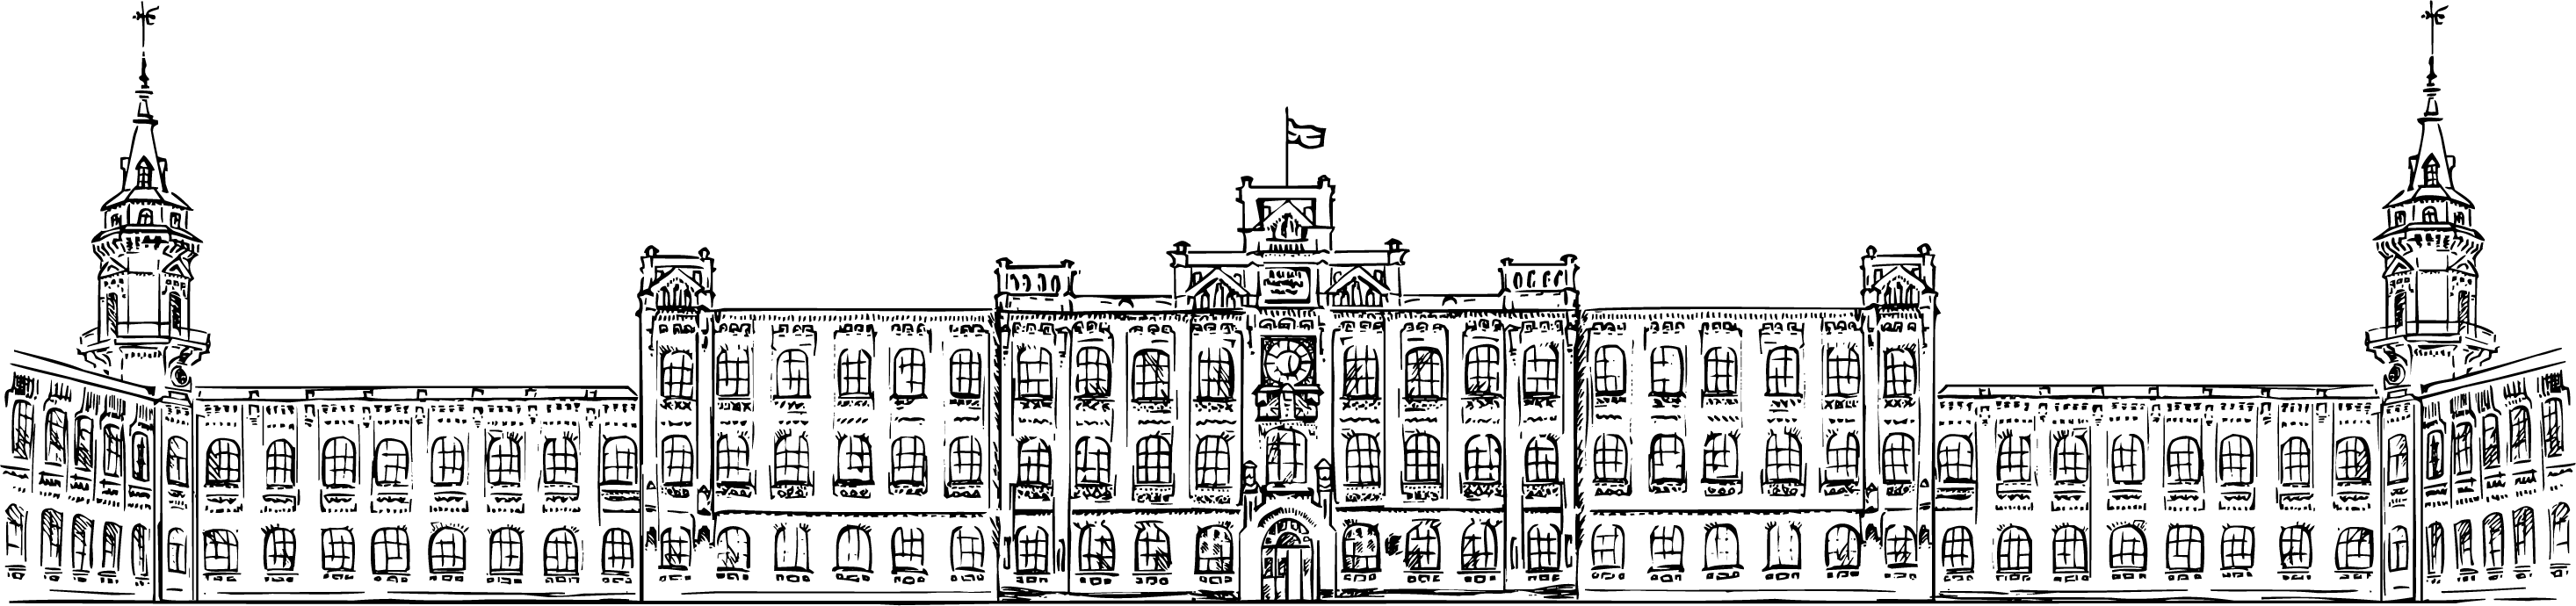
\includegraphics[width=0.7\textwidth]{../../../../../../templates/letterhead.png}
  \end{center}

  \begin{center}
    \large
    Національний технічний університет України\\
    «Київський політехнічний інститут імені Ігоря Сікорського»\\[1em]
    Факультет інформатики та обчислювальної техніки\\
    Кафедра обчислювальної техніки
  \end{center}

  \vfill

  \begin{center}
    \textbf{\LARGE Технології Computer Vision}\\[2em]
    \textbf{\Large Лабораторна робота №2}\\[0.7em]
    \parbox{0.9\textwidth}{\centering
      «Растрові та векторні цифрові зображення»}
  \end{center}

  \vfill

  \begin{flushright}
    \begin{minipage}{0.48\textwidth}
      Виконав: студент 3 курсу ФІОТ,\\
      групи \studentGroup\\
      \textit{\studentName}\\
      Залікова книжка № \recordBook\\[1em]
      Перевірив: \textit{\teacherName}
    \end{minipage}
  \end{flushright}

  \vfill
  \begin{center}Київ --- \reportYear\end{center}
\end{titlepage}

\pagenumbering{arabic}
\setlength{\parindent}{1.25cm}

\section{Тема та мета роботи}

\noindent
\textbf{Тема:} дослідження растрових і векторних цифрових зображень, а також підготовка зображень для виявлення об'єктів за їхніми контурами.

\medskip

\noindent
\textbf{Мета:} дослідити практичне застосування методів попередньої обробки растрових зображень, бінаризації, виділення контурів і геометричної фільтрації для виявлення будівель на знімках однієї території.

\section{Завдання роботи}

У лабораторній роботі реалізовано програмний pipeline для аналізу двох зображень однієї території. Основні завдання:

\begin{enumerate}[leftmargin=*,itemsep=0.25em]
  \item завантажити два растрові зображення та дослідити їхню якість;
  \item виконати перетворення зображень у відтінки сірого та розмиття;
  \item дослідити бінаризацію методом Otsu та адаптивну бінаризацію;
  \item реалізувати пошук контурів методом Canny та за бінарною маскою;
  \item сформувати кольорову маску для виділення світлих малонасичених ділянок, характерних для дахів;
  \item відфільтрувати контури за площею, співвідношенням сторін і заповненістю обмежувального прямокутника;
  \item вирівняти два зображення за ключовими точками ORB і знайти стабільні області, що підтверджуються на обох знімках;
  \item порівняти pipeline та визначити найкращу комбінацію операцій.
\end{enumerate}

\section{Математична модель}

\subsection{Растрове зображення та grayscale}

Растрове зображення подано як тривимірний масив:

\begin{equation}
  I \in \{0,\ldots,255\}^{H \times W \times 3},
\end{equation}

де \(H\) і \(W\) --- висота та ширина зображення, а третій індекс відповідає колірним каналам. Для переходу до відтінків сірого використовується зважена сума каналів:

\begin{equation}
  G(x,y)=0.299R(x,y)+0.587G(x,y)+0.114B(x,y).
\end{equation}

Відтінки сірого зменшують розмірність задачі: замість трьох значень кольору для кожного пікселя використовується одна яскравість.

\subsection{Гаусове розмиття}

Перед виділенням контурів зображення згладжується. У програмі використовується \texttt{GaussianBlur} з ядром \(5\times5\). Загальна формула двовимірного гаусового ядра має вигляд:

\begin{equation}
  K_\sigma(x,y)=\frac{1}{2\pi\sigma^2}
  \exp\left(-\frac{x^2+y^2}{2\sigma^2}\right).
\end{equation}

Результат згладжування обчислюється згорткою \(G*K_\sigma\). Це зменшує вплив дрібного шуму та текстур, які можуть створювати зайві контури.

\subsection{Глобальна та адаптивна бінаризація}

Після grayscale формується бінарна маска:

\begin{equation}
  B(x,y)=
  \begin{cases}
    255, & G(x,y)>T,\\
    0, & G(x,y)\leq T.
  \end{cases}
\end{equation}

У методі Otsu поріг \(T\) вибирається автоматично. Він максимізує міжкласову дисперсію яскравостей, тобто намагається розділити пікселі фону й об'єктів.

Адаптивна бінаризація використовує локальний поріг:

\begin{equation}
  B(x,y)=
  \begin{cases}
    255, & G(x,y)>\mu_{\mathcal{N}(x,y)}-C,\\
    0, & G(x,y)\leq\mu_{\mathcal{N}(x,y)}-C.
  \end{cases}
\end{equation}

де \(\mu_{\mathcal{N}(x,y)}\) --- середня яскравість у локальному вікні, а \(C\) --- стала поправка. Такий метод може виділяти об'єкти при нерівномірному освітленні, але на супутникових знімках часто створює багато локального шуму.

\subsection{Кольорова маска}

Для пошуку дахів використовується маска світлих малонасичених пікселів. Для каналів \(R,G,B\) піксель приймається, якщо:

\begin{equation}
  |R-G|\leq c, \qquad |G-B|\leq c,
  \qquad R\geq v,\;G\geq v,\;B\geq v,
\end{equation}

де \(c\) --- допустима різниця каналів, а \(v\) --- мінімальна яскравість. Така маска не розпізнає будівлю семантично, але добре виділяє світлі та сірі поверхні дахів.

\subsection{Контури та геометрична фільтрація}

Для кожної бінарної маски алгоритм \texttt{findContours} формує набір контурів \(C_i\). Для контуру обчислюються площа \(A_i\), обмежувальний прямокутник \(w_i\times h_i\), співвідношення сторін та заповненість:

\begin{equation}
  r_i=\frac{w_i}{h_i}, \qquad
  e_i=\frac{A_i}{w_i h_i}.
\end{equation}

Контур приймається, якщо виконується система обмежень:

\begin{equation}
  A_{\min}\leq A_i\leq A_{\max},\qquad
  r_{\min}\leq r_i\leq r_{\max},\qquad
  e_i\geq e_{\min}.
\end{equation}

Площа нормується відносно площі всього зображення:

\begin{equation}
  A_{\min}=\rho_{\min}HW, \qquad
  A_{\max}=\rho_{\max}HW.
\end{equation}

Так фільтр не залежить безпосередньо від абсолютної роздільної здатності знімка.

\subsection{Вирівнювання двох зображень}

Оскільки два зображення описують одну територію, вони вирівнюються за ключовими точками ORB. За відповідностями точок оцінюється гомографія:

\begin{equation}
  \begin{bmatrix}x'\\y'\\1\end{bmatrix}
  \sim
  H
  \begin{bmatrix}x\\y\\1\end{bmatrix},
  \qquad H\in\mathbb{R}^{3\times3}.
\end{equation}

Викиди відкидаються методом RANSAC. Після перенесення кольорової маски другого зображення до координат першого формується перетин:

\begin{equation}
  M_{\mathrm{stable}}=M_1\cap\operatorname{warp}(M_2,H).
\end{equation}

Таким чином, залишаються області, які одночасно виявлені на двох знімках.

\section{Архітектура та алгоритми}

Загальна архітектура програмного рішення має вигляд:

\begin{figure}[H]
  \centering
  \begin{tikzpicture}[
    node distance=0.65cm and 1.2cm,
    block/.style={draw, rounded corners, align=center, minimum width=3.8cm, minimum height=0.85cm, fill=blue!7},
    arrow/.style={-{Latex[length=2mm]}, thick}
  ]
    \node[block] (input) {Два растрові\\зображення};

    \node[block, below left=1.0cm and 1.8cm of input] (independent)
      {Незалежний аналіз\\кожного зображення};
    \node[block, below right=1.0cm and 1.8cm of input] (pair)
      {Спільний аналіз\\пари зображень};

    \node[block, below=of independent] (preprocess)
      {Grayscale, Blur\\та маски};
    \node[block, below=of preprocess] (contours)
      {findContours\\та геометрична фільтрація};
    \node[block, below=of contours] (count)
      {Підрахунок контурів\\для кожного фото};

    \node[block, below=of pair] (registration)
      {ORB, гомографія\\та warpPerspective};
    \node[block, below=of registration] (intersection)
      {Перетин масок\\та морфологічне closing};
    \node[block, below=of intersection] (stable)
      {Стабільні контури\\та підрахунок};

    \draw[arrow] (input.south) -- (independent.north);
    \draw[arrow] (input.south) -- (pair.north);
    \draw[arrow] (independent) -- (preprocess);
    \draw[arrow] (preprocess) -- (contours);
    \draw[arrow] (contours) -- (count);
    \draw[arrow] (pair) -- (registration);
    \draw[arrow] (registration) -- (intersection);
    \draw[arrow] (intersection) -- (stable);
  \end{tikzpicture}
  \caption{Блок-схема програмного pipeline}
\end{figure}

Основні програмні компоненти наведено в таблиці.

\setlength{\LTleft}{0pt}
\setlength{\LTright}{0pt}
\renewcommand{\arraystretch}{1.2}
\begin{longtable}{|p{5.4cm}|p{9.0cm}|}
  \caption{Компоненти програмного рішення}\label{tab:components}\\
  \hline
  \textbf{Компонент} & \textbf{Призначення} \\
  \hline
  \endfirsthead
  \hline
  \textbf{Компонент} & \textbf{Призначення} \\
  \hline
  \endhead
  \texttt{load\_image} & Завантаження зображення у форматі BGR. \\
  \hline
  \texttt{detect\_by\_canny} & Згладжування, Canny та пошук зовнішніх контурів. \\
  \hline
  \texttt{detect\_by\_threshold} & Grayscale, Otsu threshold та пошук контурів. \\
  \hline
  \begin{tabular}[t]{@{}l@{}}\texttt{detect\_by\_adaptive\_}\\\texttt{threshold}\end{tabular} & Локальна бінаризація з адаптивним порогом. \\
  \hline
  \texttt{detect\_by\_color\_mask} & Виділення світлих малонасичених ділянок. \\
  \hline
  \texttt{filter\_contours} & Фільтрація контурів за площею та геометрією. \\
  \hline
  \texttt{estimate\_homography} & Вирівнювання двох зображень за ORB-відповідностями. \\
  \hline
  \begin{tabular}[t]{@{}l@{}}\texttt{detect\_registered\_}\\\texttt{color\_consensus}\end{tabular} & Перетин масок після просторового вирівнювання. \\
  \hline
  \texttt{draw\_results} & Відображення контурів, номерів і збереження результату. \\
  \hline
\end{longtable}

\subsection{Алгоритм незалежного аналізу зображення}

\begin{enumerate}[leftmargin=*,itemsep=0.25em]
  \item Завантажити зображення.
  \item Побудувати grayscale та розмите зображення.
  \item Запустити Canny, Otsu threshold, adaptive threshold і кольорову маску.
  \item Для кожної маски знайти зовнішні контури.
  \item Відкинути контури, що не проходять геометричні обмеження.
  \item Намалювати прийняті контури та вивести їхню кількість.
\end{enumerate}

\subsection{Алгоритм зареєстрованого консенсусу}

\begin{enumerate}[leftmargin=*,itemsep=0.25em]
  \item Визначити ключові точки ORB на двох зображеннях.
  \item Зіставити дескриптори та залишити відповідності за ratio test.
  \item Оцінити гомографію RANSAC.
  \item Побудувати кольорову маску для кожного зображення.
  \item Перенести маску другого зображення в систему координат першого.
  \item Обчислити перетин масок, виконати морфологічне замикання.
  \item Відфільтрувати контури та вивести стабільні кандидати.
\end{enumerate}

\section{Структура проєкту}

У папці лабораторної роботи розміщено:

\begin{itemize}[leftmargin=*,itemsep=0.25em]
  \item \texttt{src/main.py} --- основний програмний скрипт;
  \item \texttt{src/photo1.png}, \texttt{src/photo2.png} --- два досліджувані зображення;
  \item \texttt{results/photo1/} і \texttt{results/photo2/} --- результати незалежного аналізу;
  \item \texttt{results/registered\_pair/} --- результати вирівнювання і спільного аналізу;
  \item \texttt{requirements.txt} --- залежності Python;
  \item \texttt{docs/main.tex} --- вихідний файл звіту;
  \item \texttt{docs/main.pdf} --- скомпільований звіт.
\end{itemize}

\section{Результати виконання}

На рисунку наведено вхідні зображення, які описують одну територію з різною роздільною здатністю та різними умовами візуалізації.

\begin{figure}[H]
  \centering
  \begin{minipage}{0.48\textwidth}
    \centering
    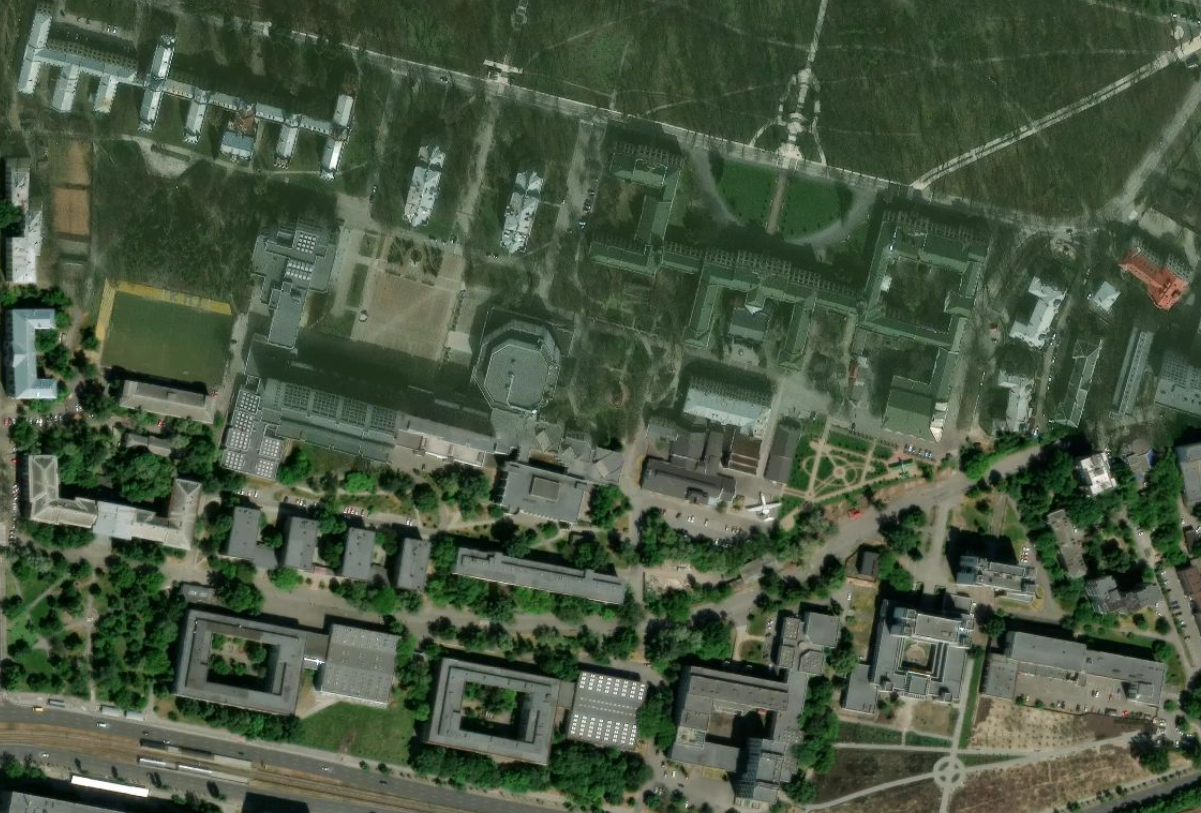
\includegraphics[width=\textwidth]{../src/photo1.png}
    \captionof{figure}{Зображення 1}
  \end{minipage}
  \hfill
  \begin{minipage}{0.48\textwidth}
    \centering
    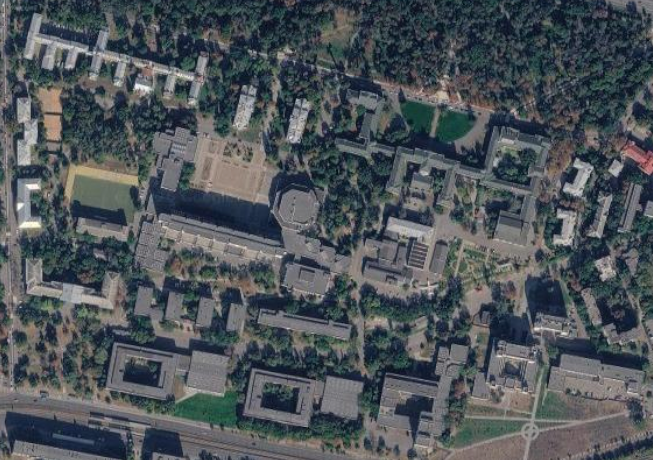
\includegraphics[width=\textwidth]{../src/photo2.png}
    \captionof{figure}{Зображення 2}
  \end{minipage}
  \caption{Вхідні растрові зображення}
\end{figure}

Кількість прийнятих контурів для окремих pipeline наведено в таблиці.

\begin{table}[H]
  \centering
  \renewcommand{\arraystretch}{1.2}
  \begin{tabular}{lrr}
    \toprule
    \textbf{Метод} & \textbf{Зображення 1} & \textbf{Зображення 2} \\
    \midrule
    Canny & 6 & 5 \\
    Otsu threshold & 37 & 24 \\
    Adaptive threshold & 10 & 11 \\
    Color mask & 38 & 30 \\
    Consensus трьох масок & 36 & 49 \\
    \bottomrule
  \end{tabular}
  \caption{Результати незалежного аналізу зображень}
\end{table}

Метод Canny у цьому випадку виявився найменш повним, оскільки формує переважно межі яскравості, а не заповнені області дахів. Глобальна бінаризація Otsu дала більше контурів, але частина з них відповідає дорогам, майданчикам і світлим ділянкам фону. Адаптивний поріг виявився нестабільним через неоднорідну текстуру супутникового зображення.

Кольорова маска краще виділяє світлі та сірі дахи. Для першого зображення використовувалися параметри \(c=15\), \(v=90\), а для другого \(c=20\), \(v=110\). Різні параметри потрібні через різну яскравість і якість зображень.

\subsection{Повний набір результатів для зображення 1}

\begin{figure}[H]
  \centering
  \begin{minipage}{0.31\textwidth}
    \centering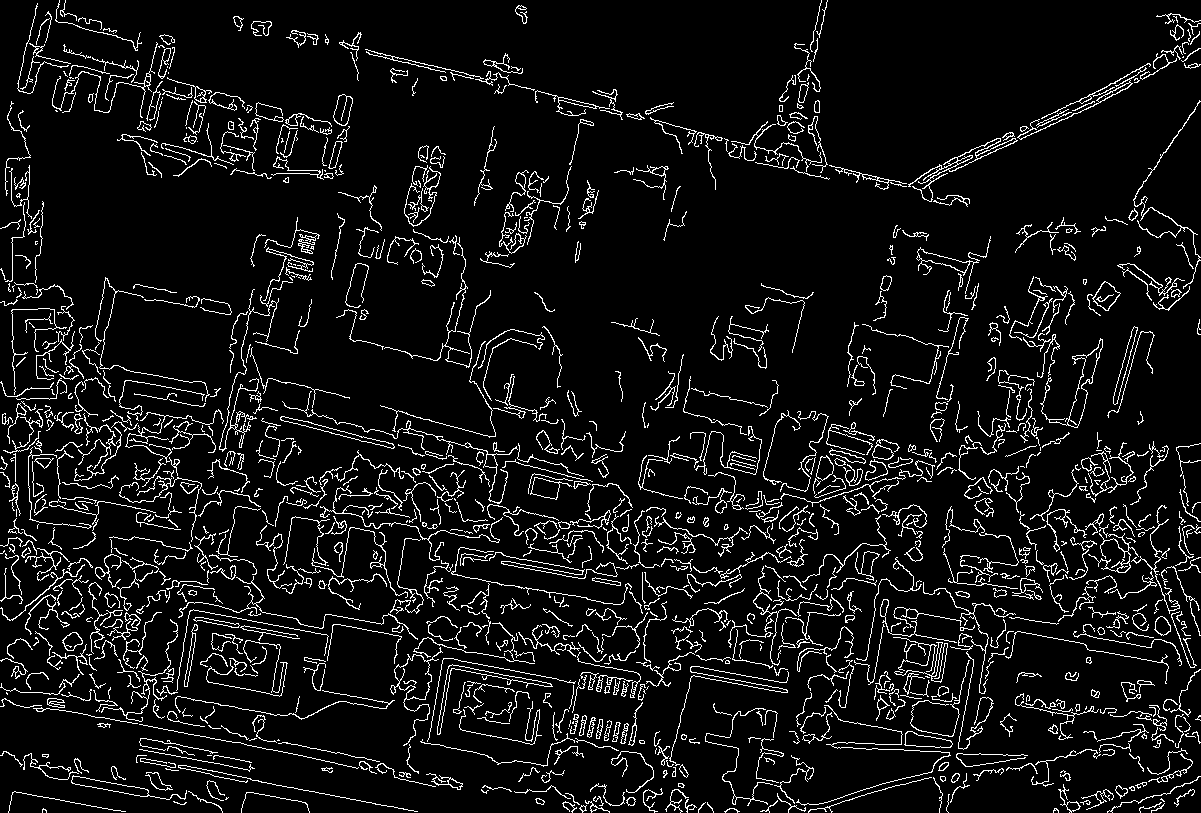
\includegraphics[width=\linewidth]{../results/photo1/canny_edges.png}\\
    \scriptsize Canny: edges
  \end{minipage}\hfill
  \begin{minipage}{0.31\textwidth}
    \centering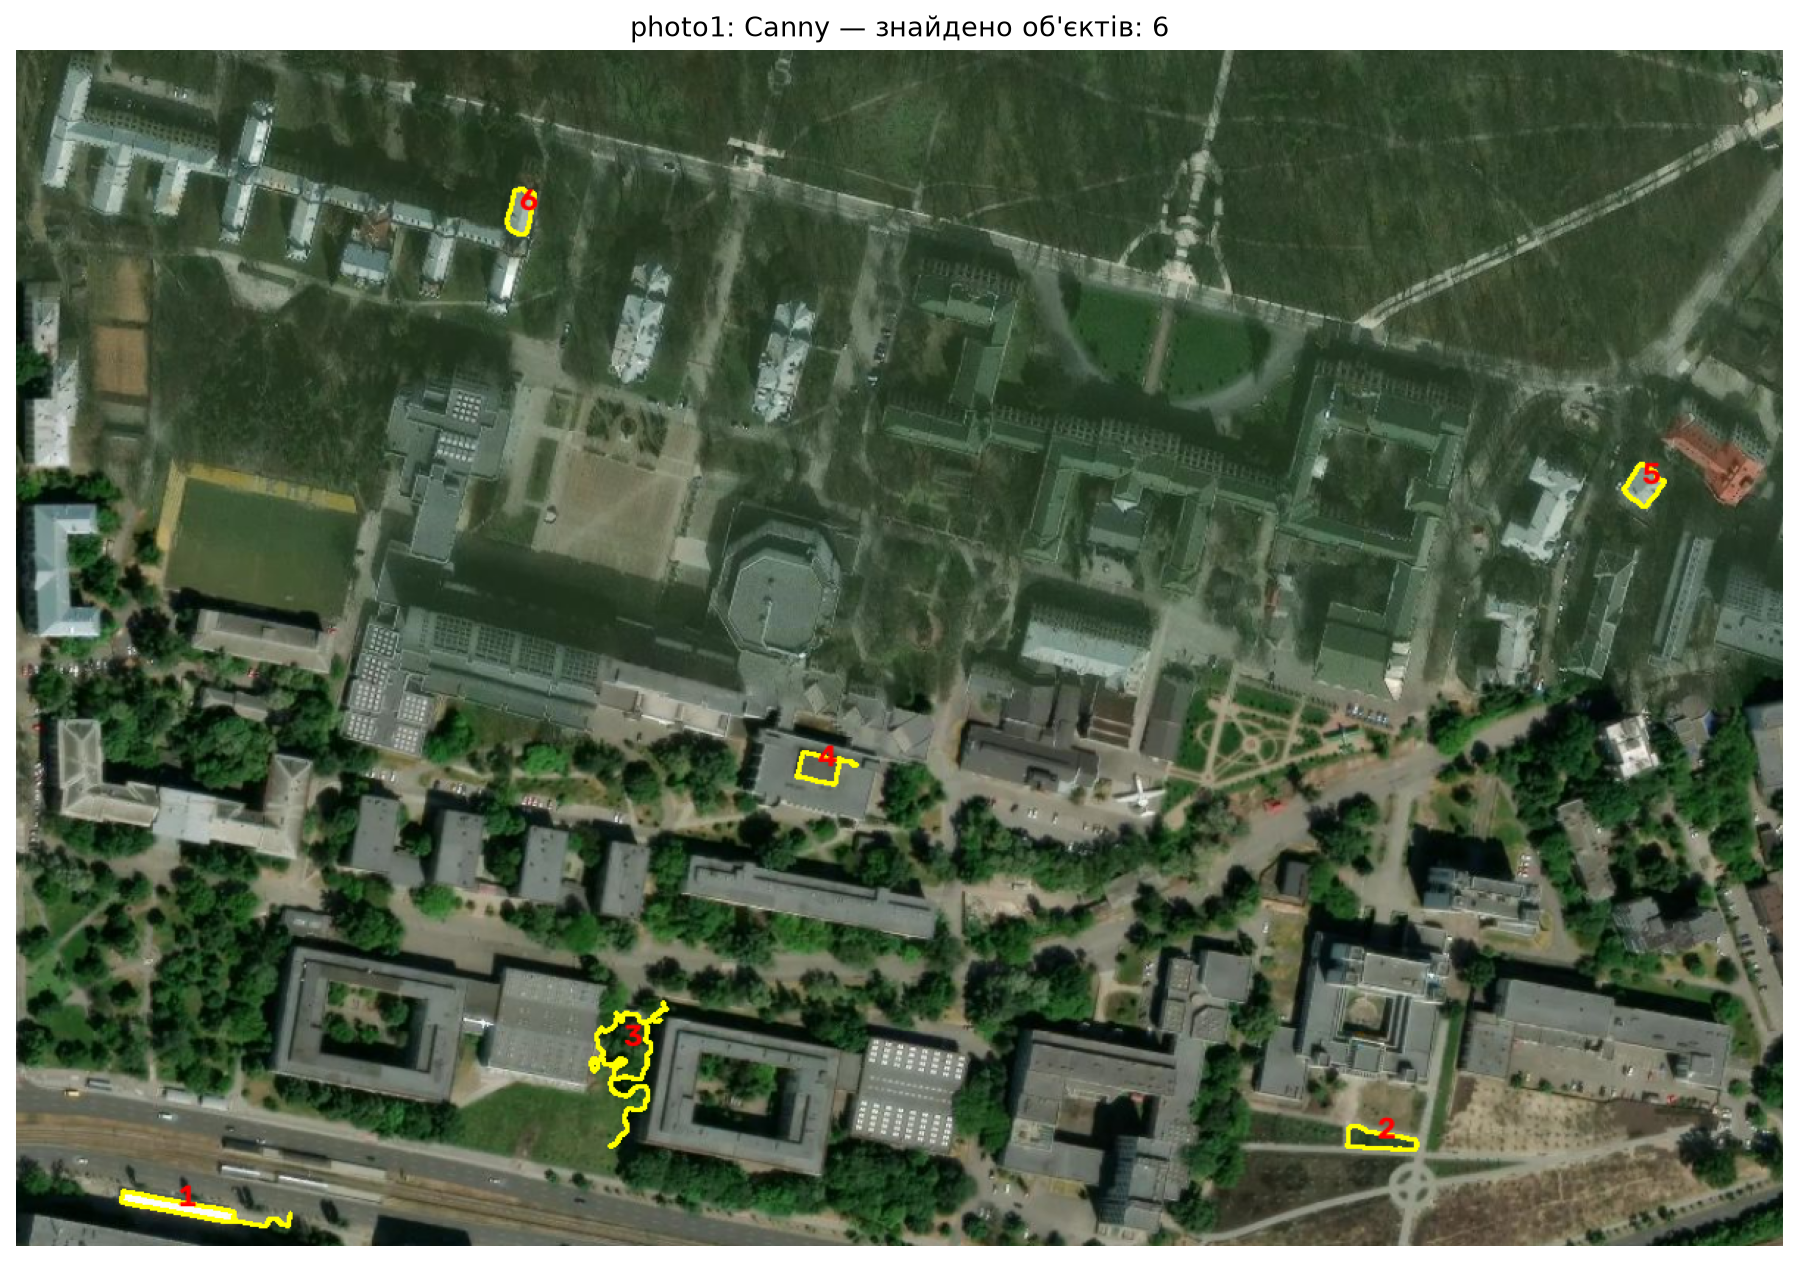
\includegraphics[width=\linewidth]{../results/photo1/canny_result.png}\\
    \scriptsize Canny: contours
  \end{minipage}\hfill
  \begin{minipage}{0.31\textwidth}
    \centering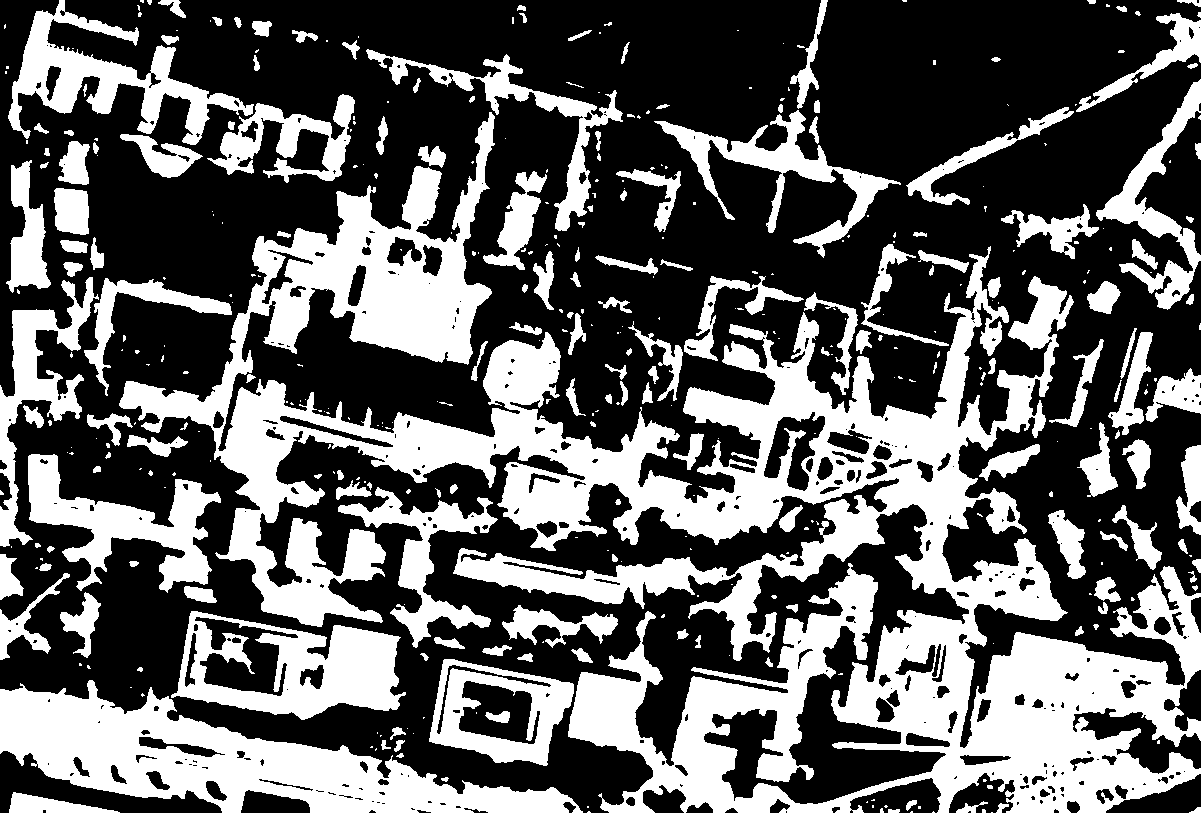
\includegraphics[width=\linewidth]{../results/photo1/threshold.png}\\
    \scriptsize Otsu: mask
  \end{minipage}

  \vspace{0.45em}
  \begin{minipage}{0.31\textwidth}
    \centering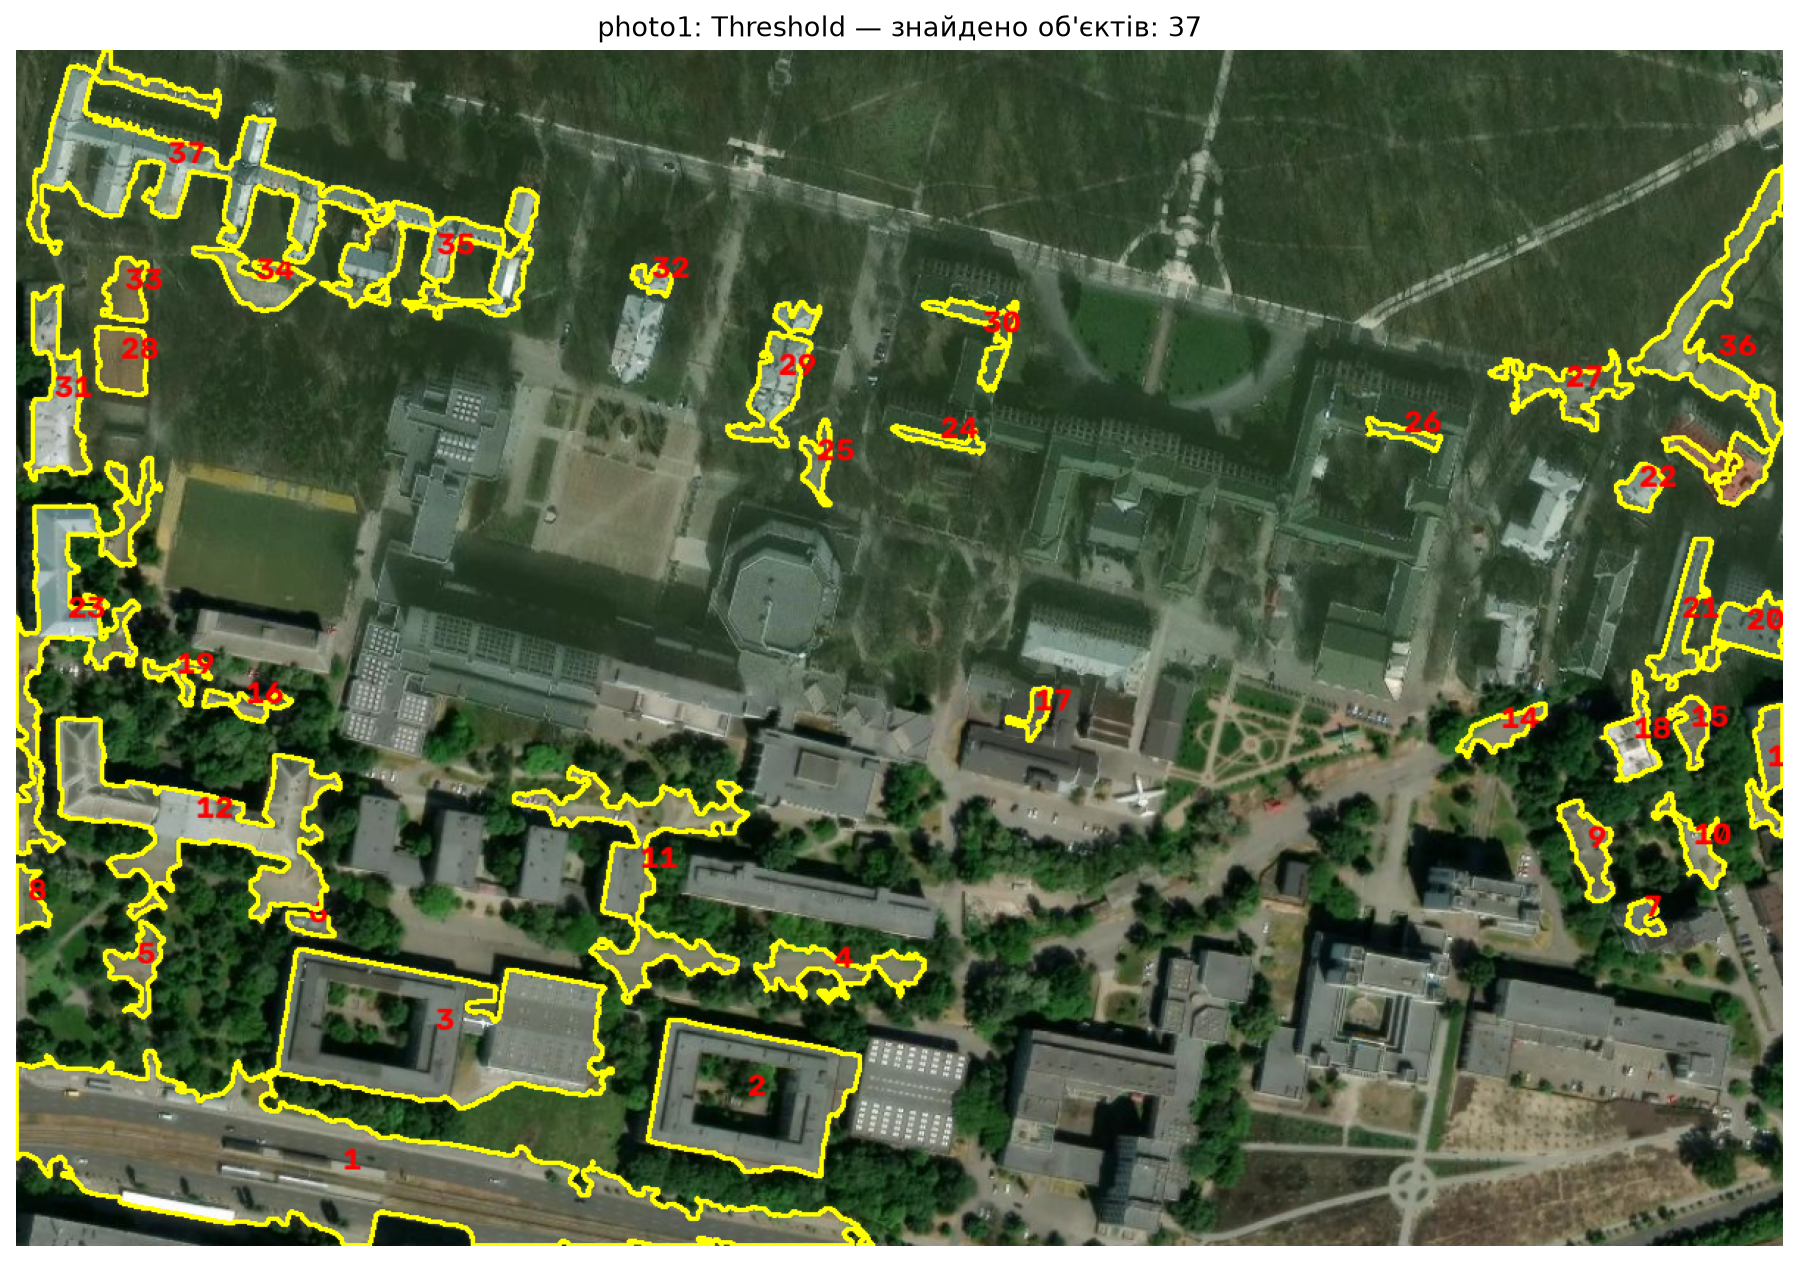
\includegraphics[width=\linewidth]{../results/photo1/threshold_result.png}\\
    \scriptsize Otsu: contours
  \end{minipage}\hfill
  \begin{minipage}{0.31\textwidth}
    \centering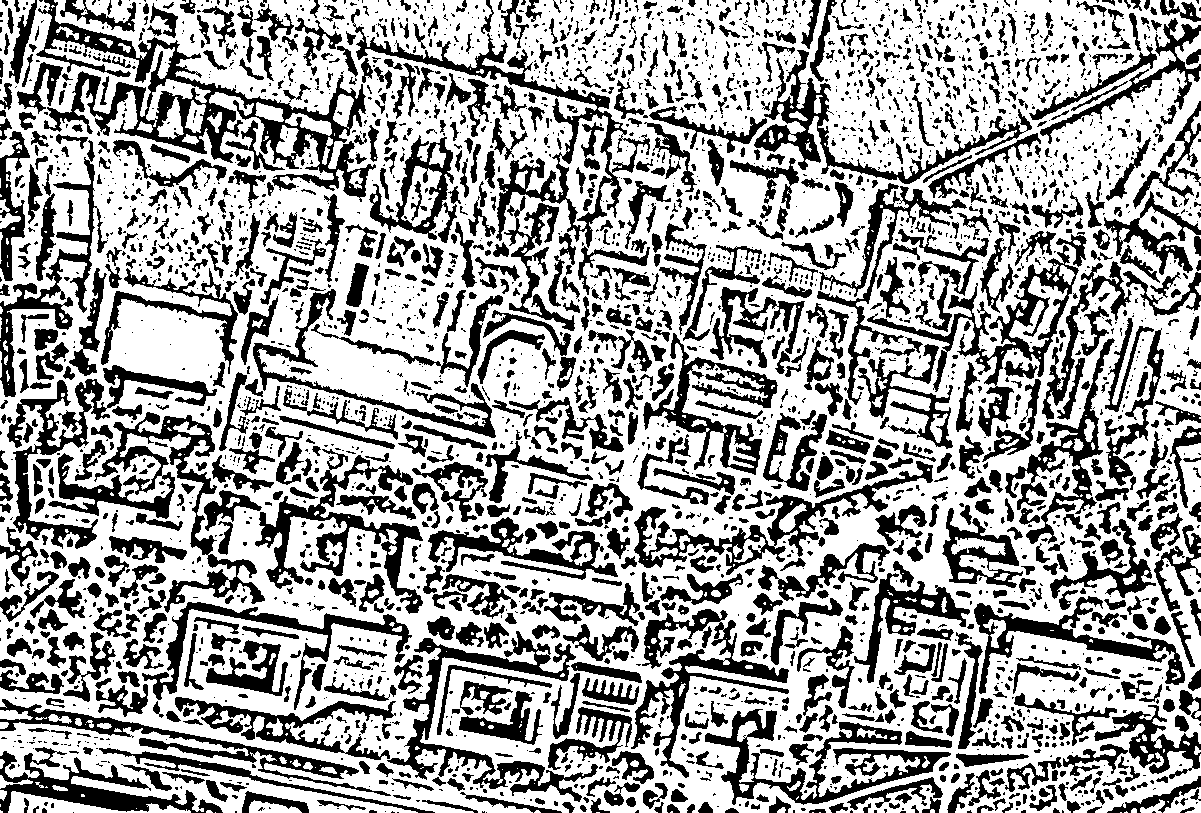
\includegraphics[width=\linewidth]{../results/photo1/adaptive_threshold.png}\\
    \scriptsize Adaptive: mask
  \end{minipage}\hfill
  \begin{minipage}{0.31\textwidth}
    \centering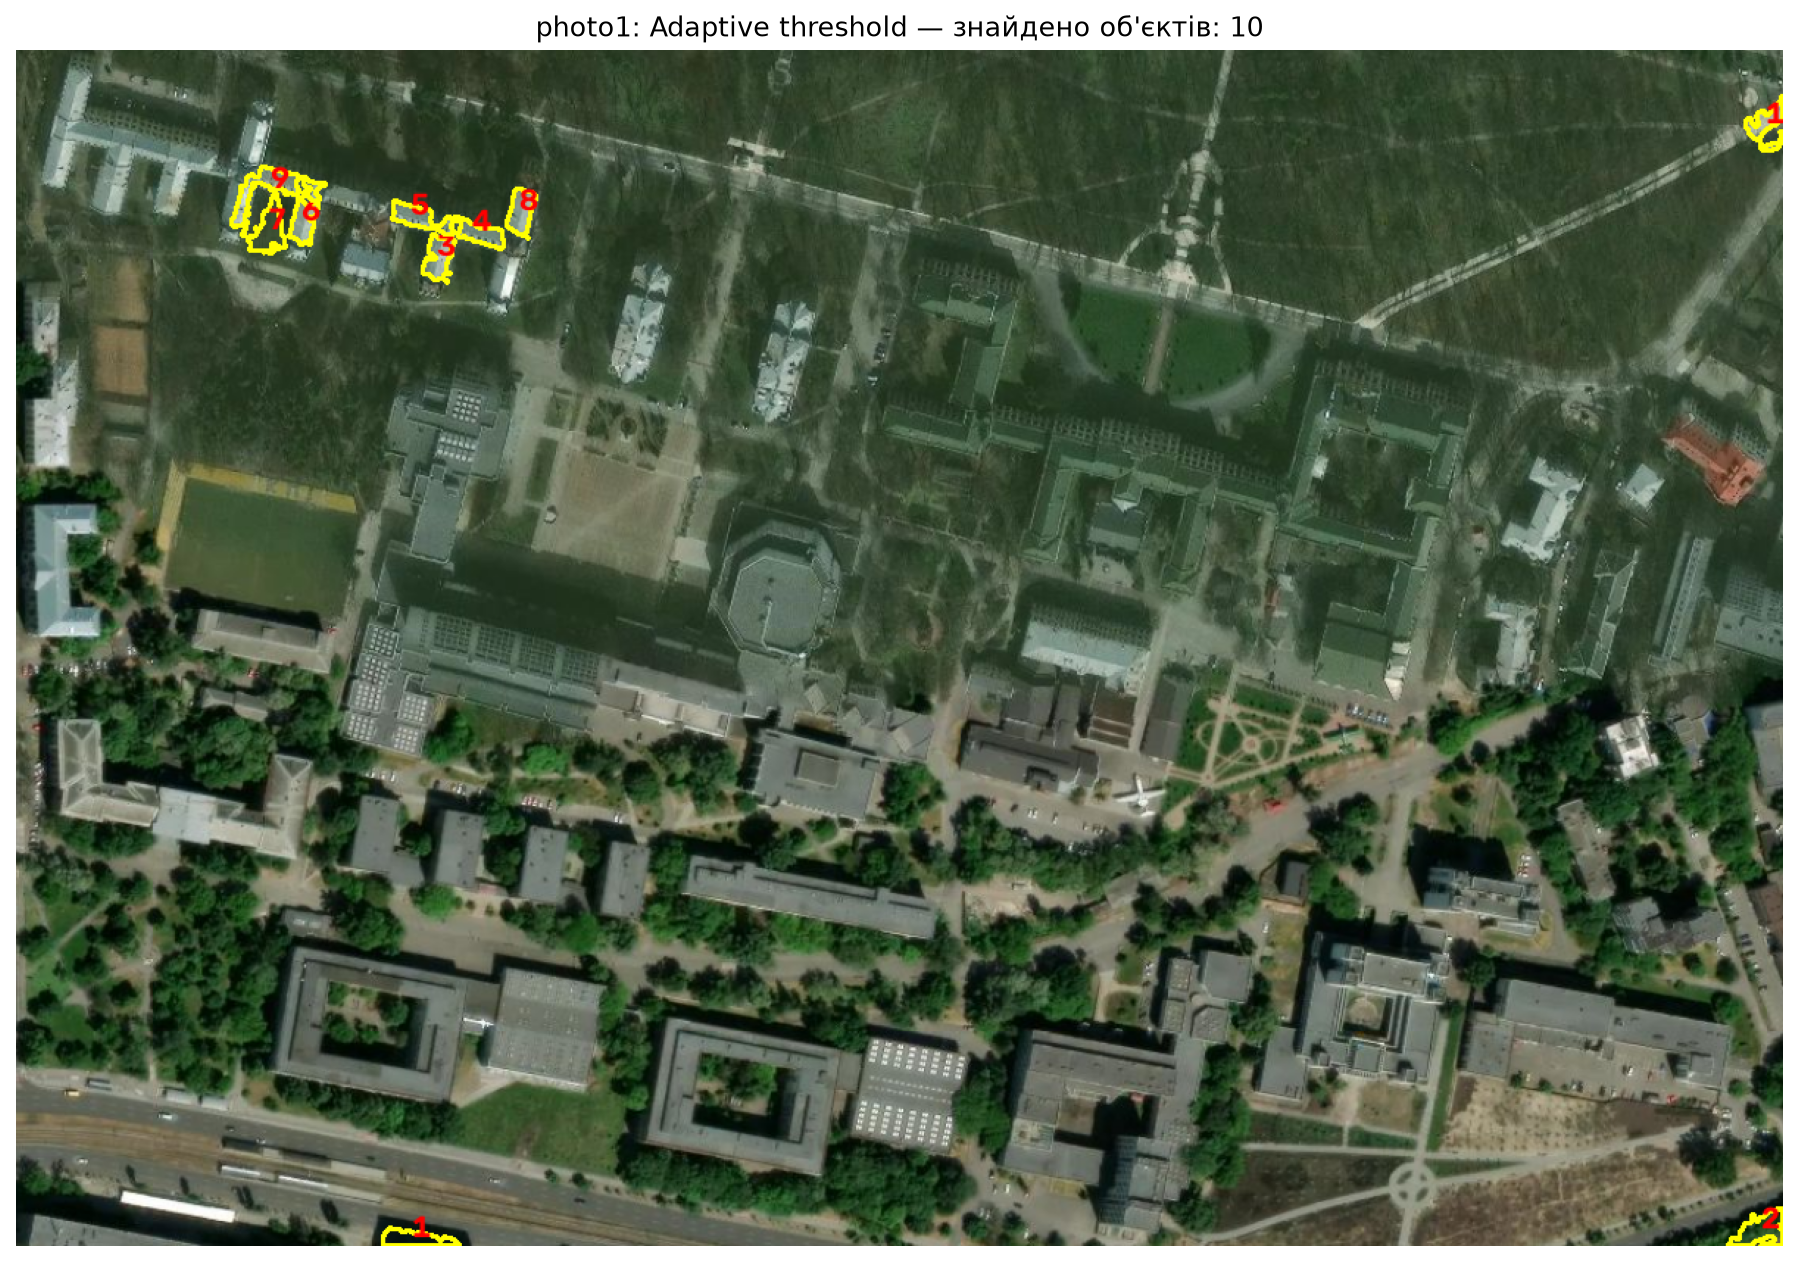
\includegraphics[width=\linewidth]{../results/photo1/adaptive_result.png}\\
    \scriptsize Adaptive: contours
  \end{minipage}

  \vspace{0.45em}
  \begin{minipage}{0.31\textwidth}
    \centering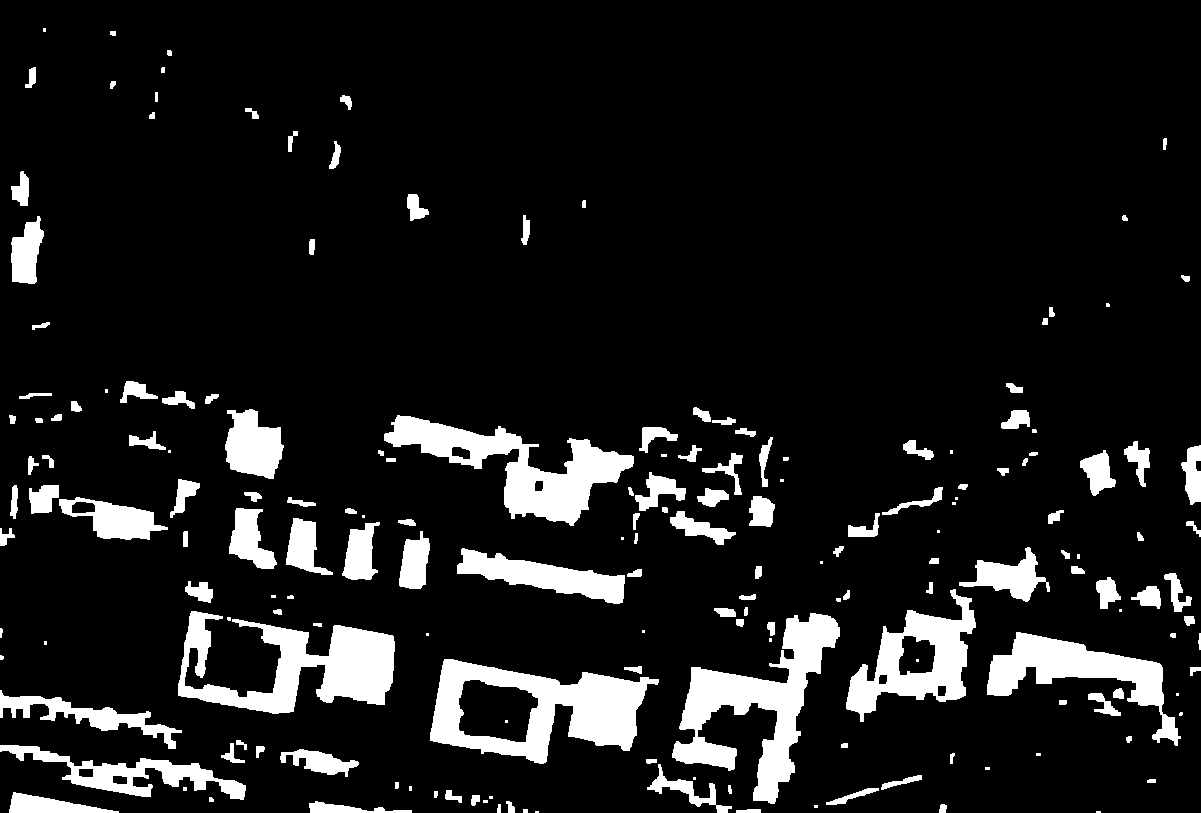
\includegraphics[width=\linewidth]{../results/photo1/color_mask.png}\\
    \scriptsize Color mask
  \end{minipage}\hfill
  \begin{minipage}{0.31\textwidth}
    \centering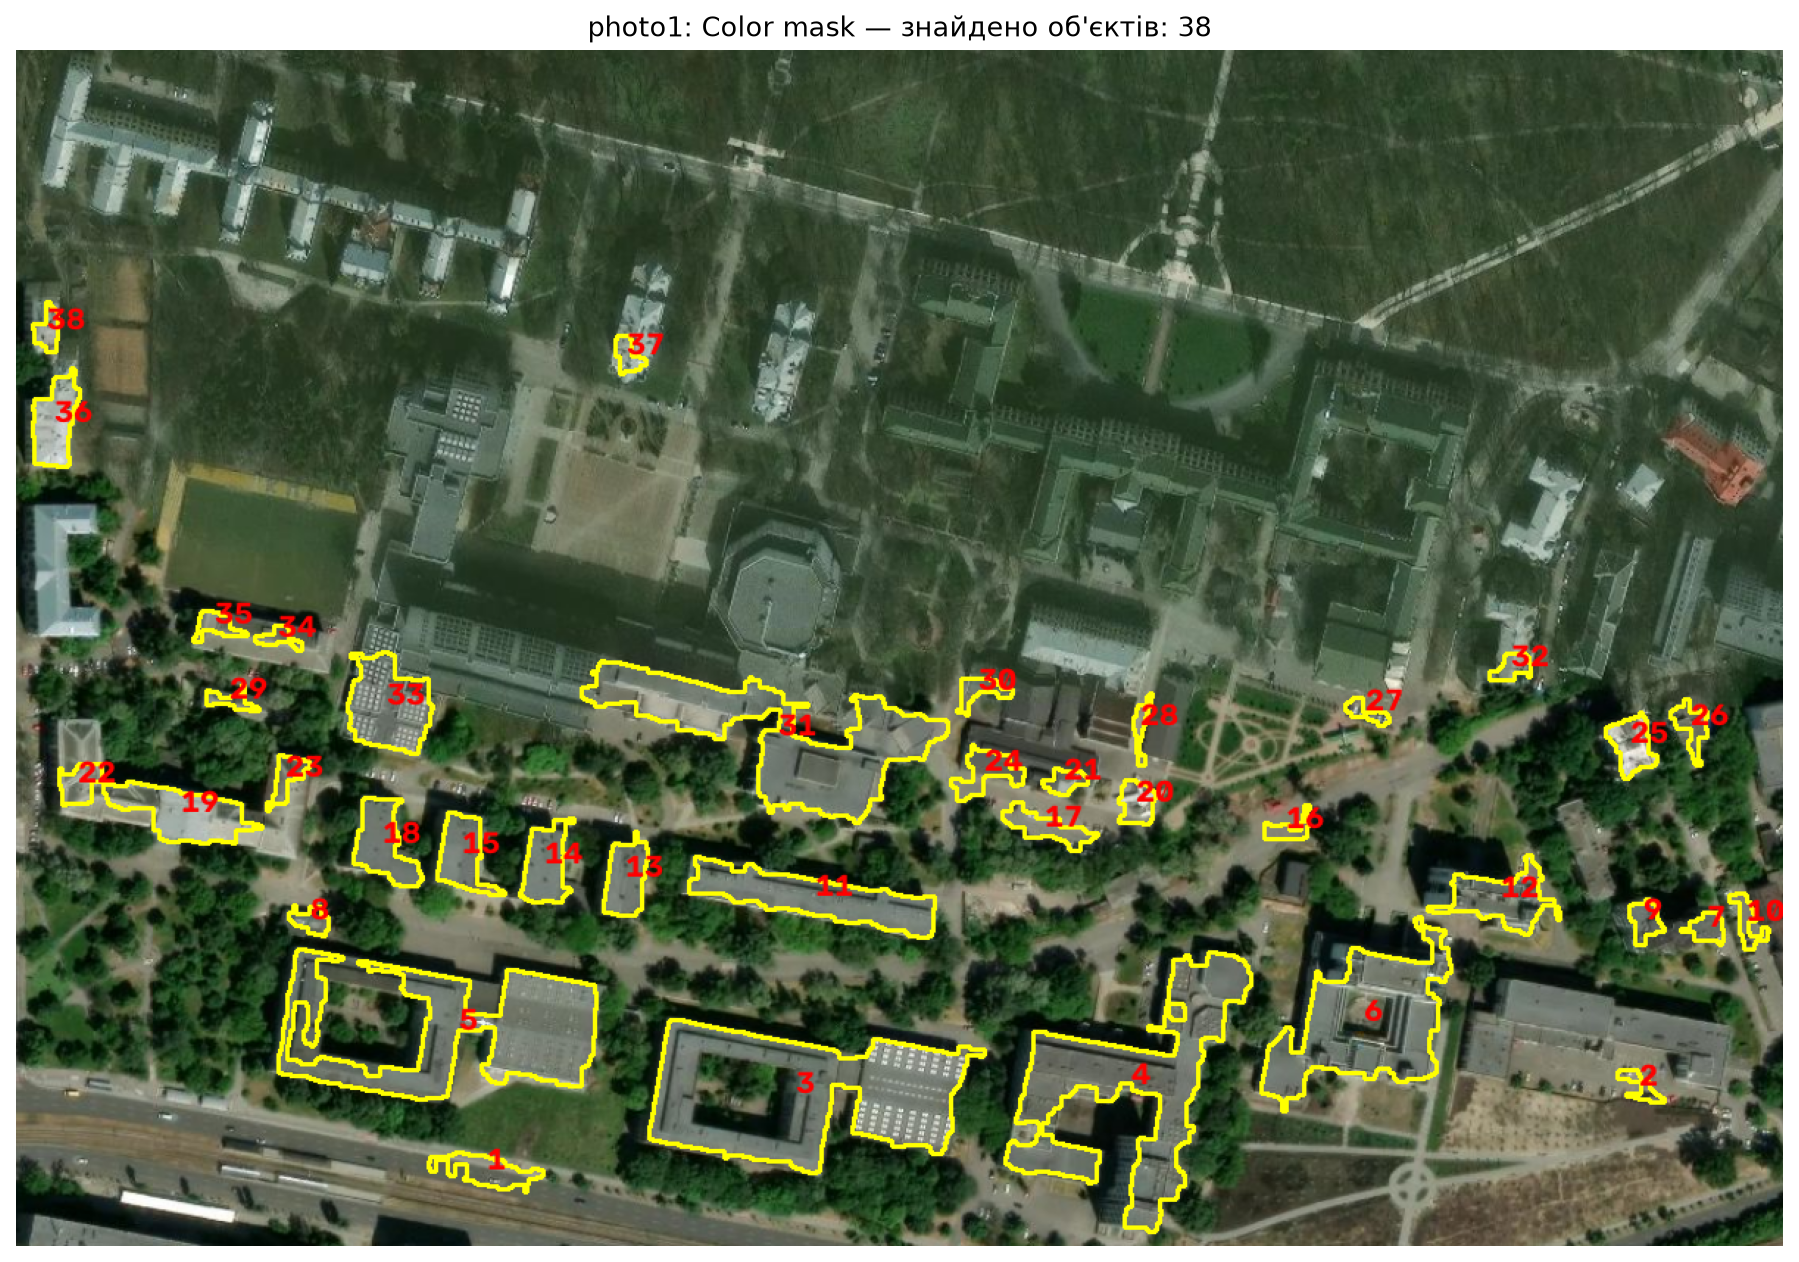
\includegraphics[width=\linewidth]{../results/photo1/color_result.png}\\
    \scriptsize Color: contours
  \end{minipage}\hfill
  \begin{minipage}{0.31\textwidth}
    \centering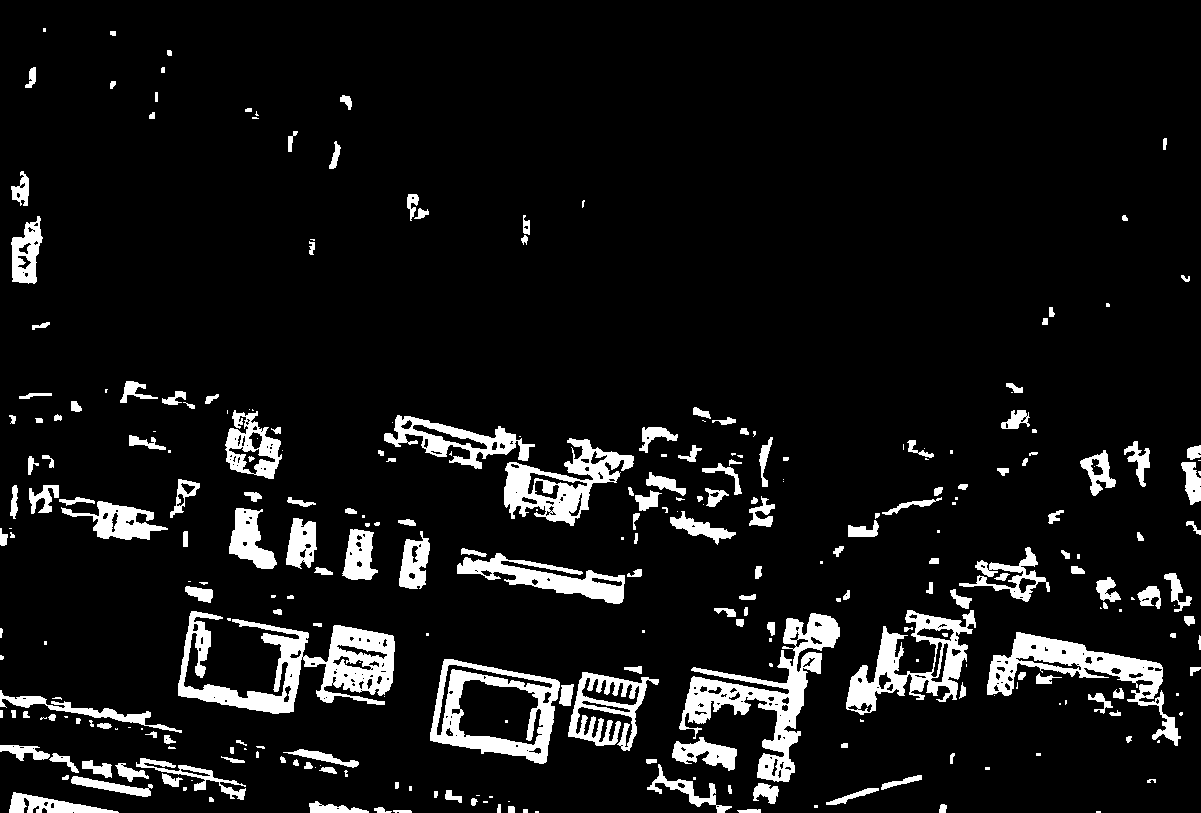
\includegraphics[width=\linewidth]{../results/photo1/consensus_mask.png}\\
    \scriptsize Consensus: mask
  \end{minipage}

  \vspace{0.45em}
  \begin{minipage}{0.31\textwidth}
    \centering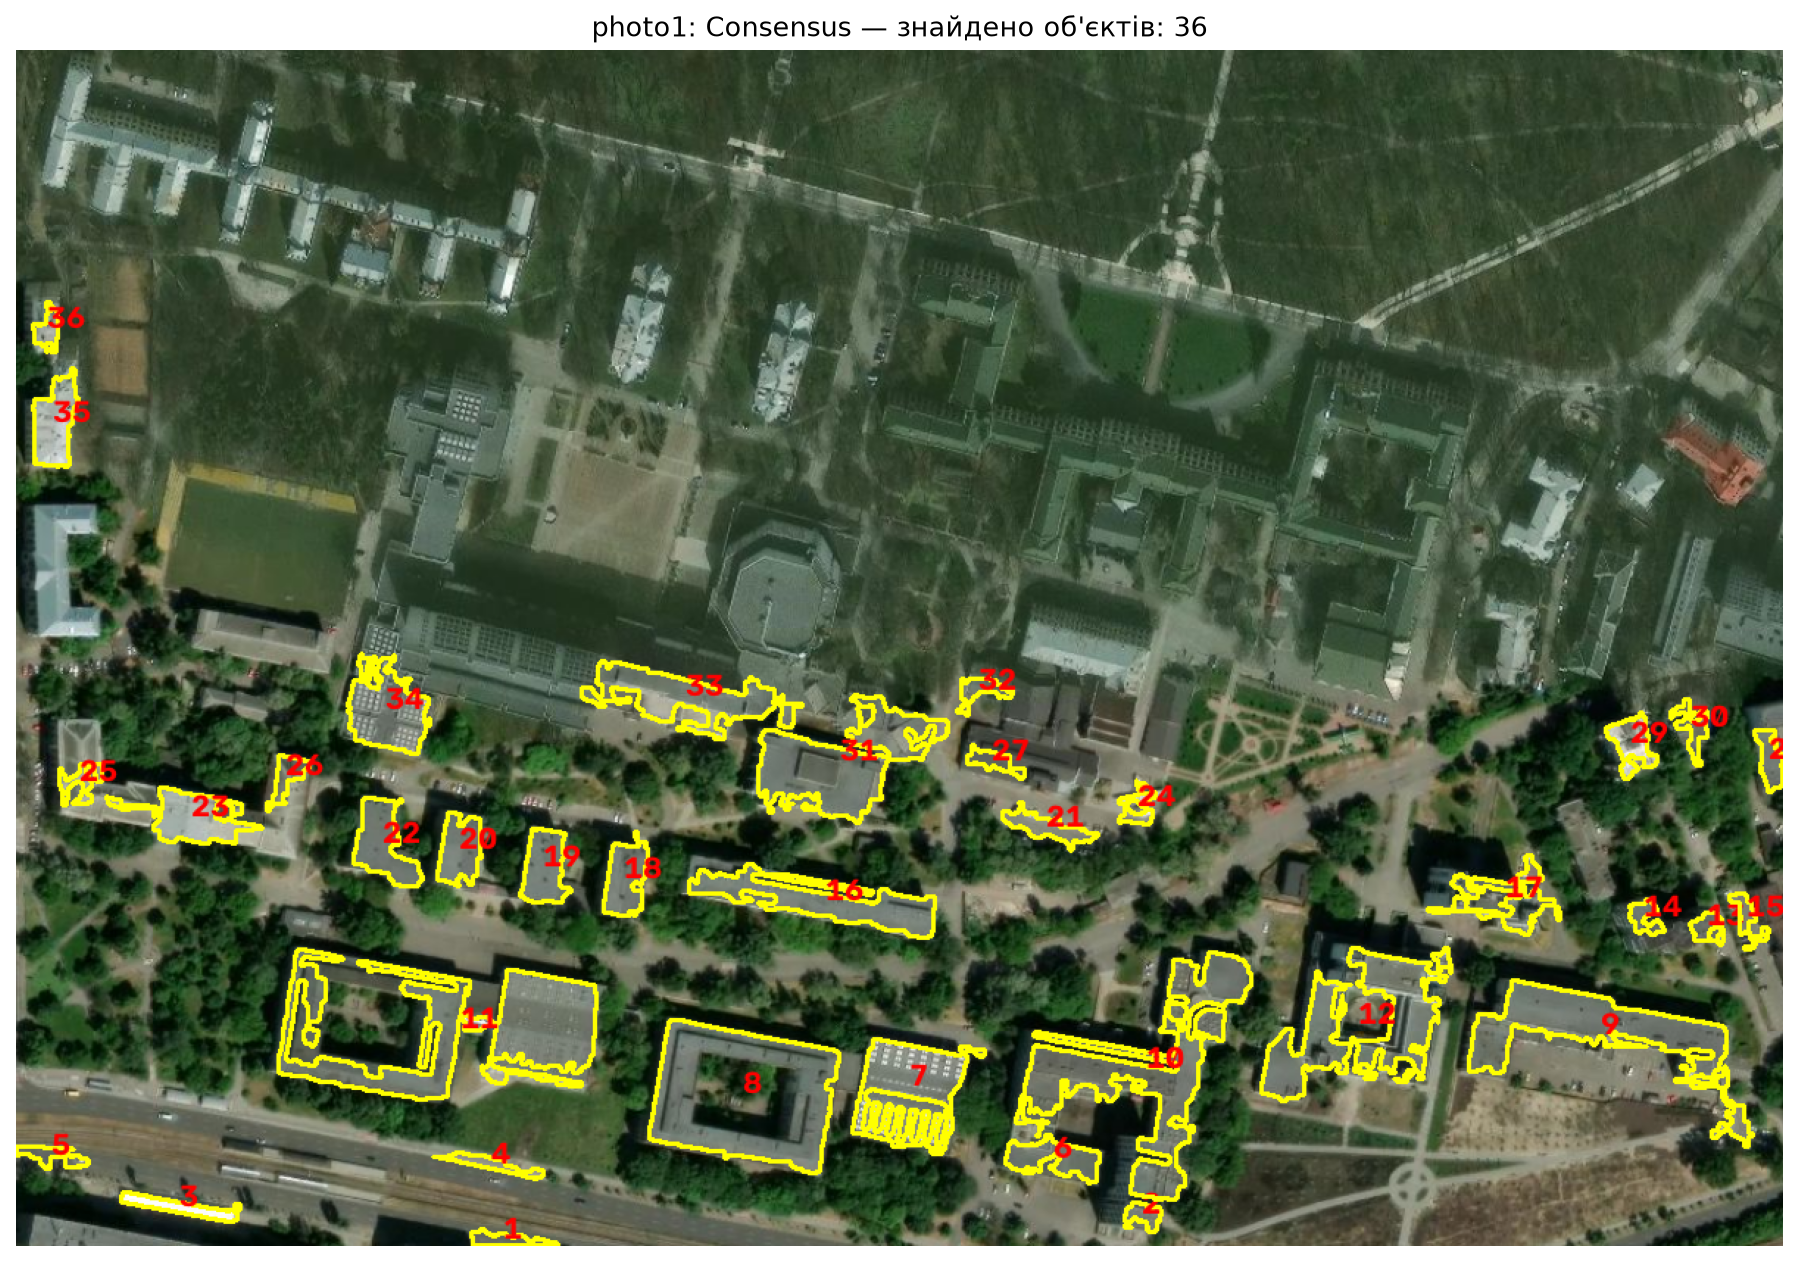
\includegraphics[width=\linewidth]{../results/photo1/consensus_result.png}\\
    \scriptsize Consensus: contours
  \end{minipage}
  \caption{Усі проміжні та фінальні результати для зображення 1}
\end{figure}

\subsection{Повний набір результатів для зображення 2}

\begin{figure}[H]
  \centering
  \begin{minipage}{0.31\textwidth}
    \centering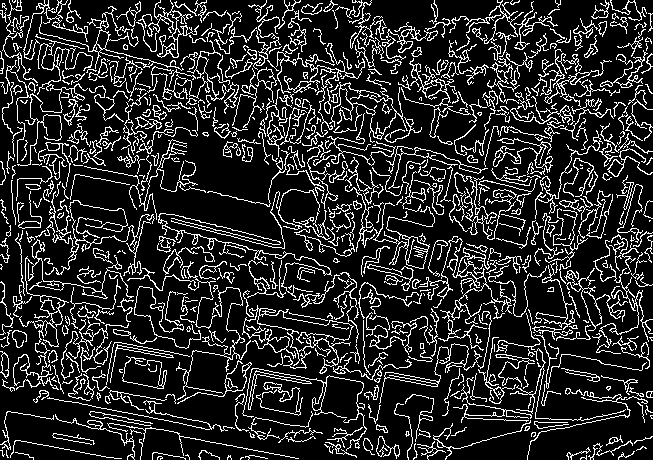
\includegraphics[width=\linewidth]{../results/photo2/canny_edges.png}\\
    \scriptsize Canny: edges
  \end{minipage}\hfill
  \begin{minipage}{0.31\textwidth}
    \centering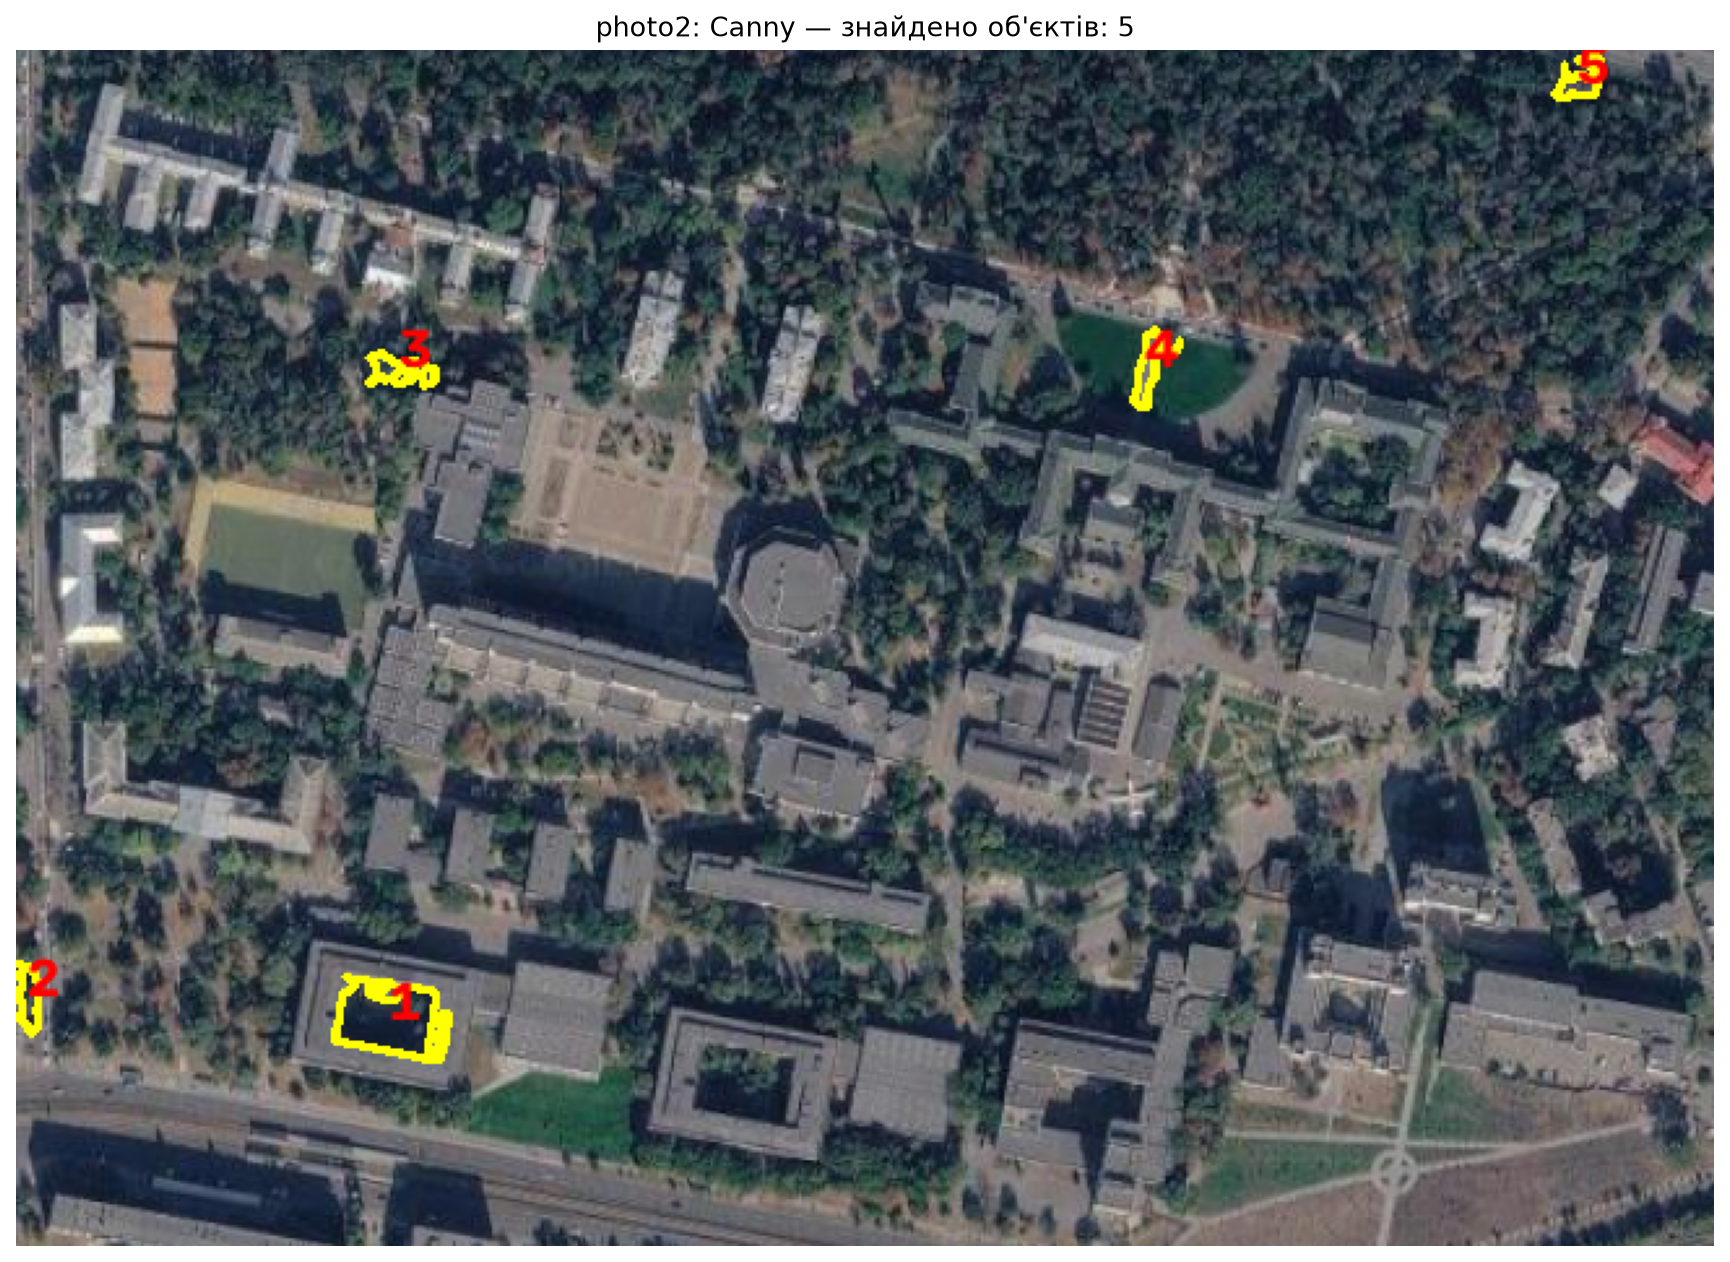
\includegraphics[width=\linewidth]{../results/photo2/canny_result.png}\\
    \scriptsize Canny: contours
  \end{minipage}\hfill
  \begin{minipage}{0.31\textwidth}
    \centering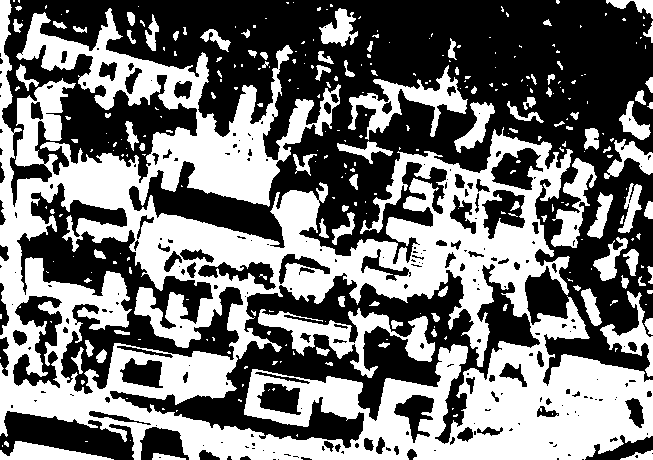
\includegraphics[width=\linewidth]{../results/photo2/threshold.png}\\
    \scriptsize Otsu: mask
  \end{minipage}

  \vspace{0.45em}
  \begin{minipage}{0.31\textwidth}
    \centering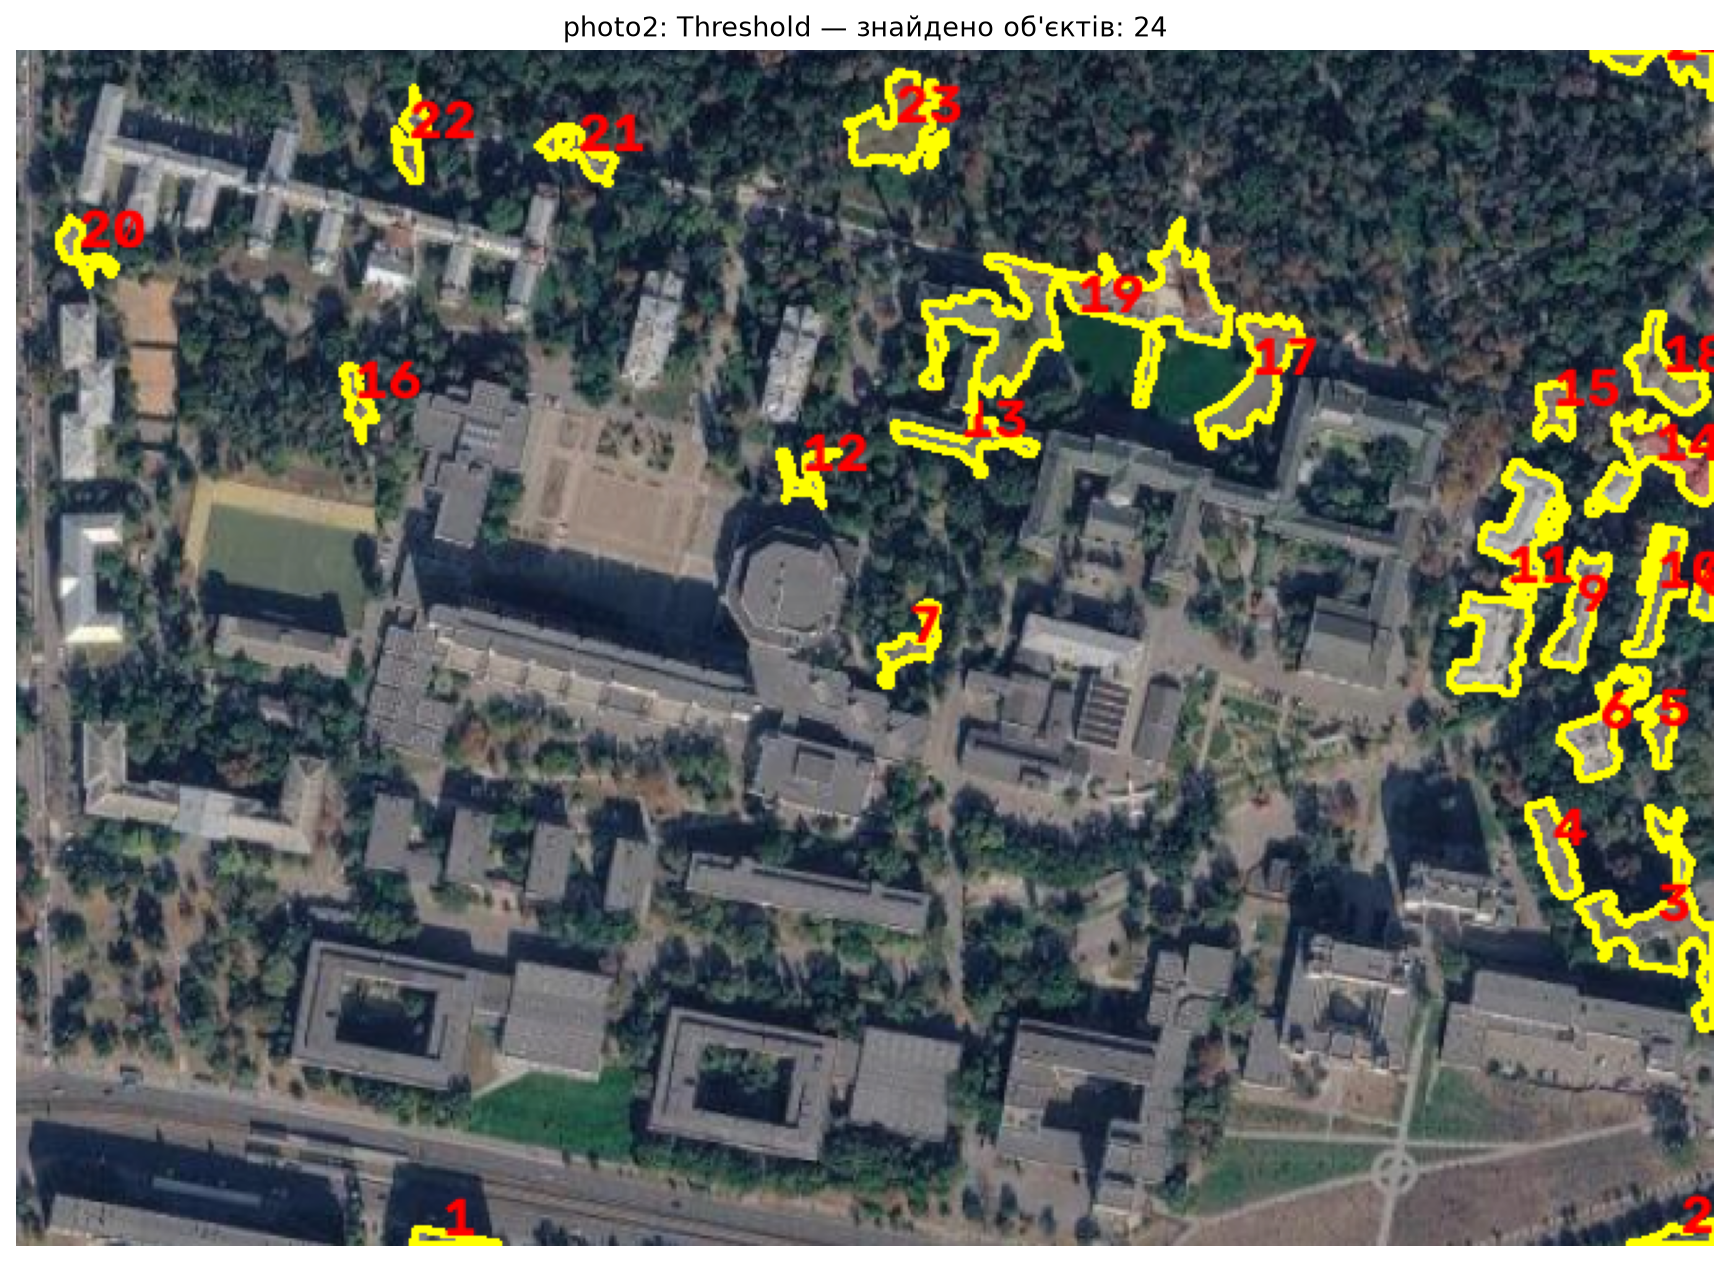
\includegraphics[width=\linewidth]{../results/photo2/threshold_result.png}\\
    \scriptsize Otsu: contours
  \end{minipage}\hfill
  \begin{minipage}{0.31\textwidth}
    \centering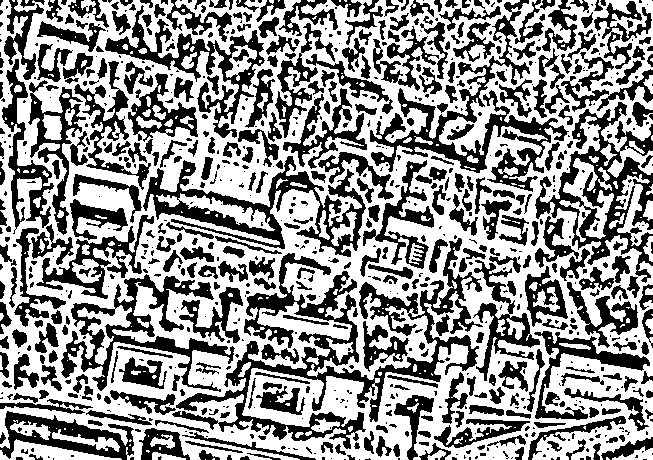
\includegraphics[width=\linewidth]{../results/photo2/adaptive_threshold.png}\\
    \scriptsize Adaptive: mask
  \end{minipage}\hfill
  \begin{minipage}{0.31\textwidth}
    \centering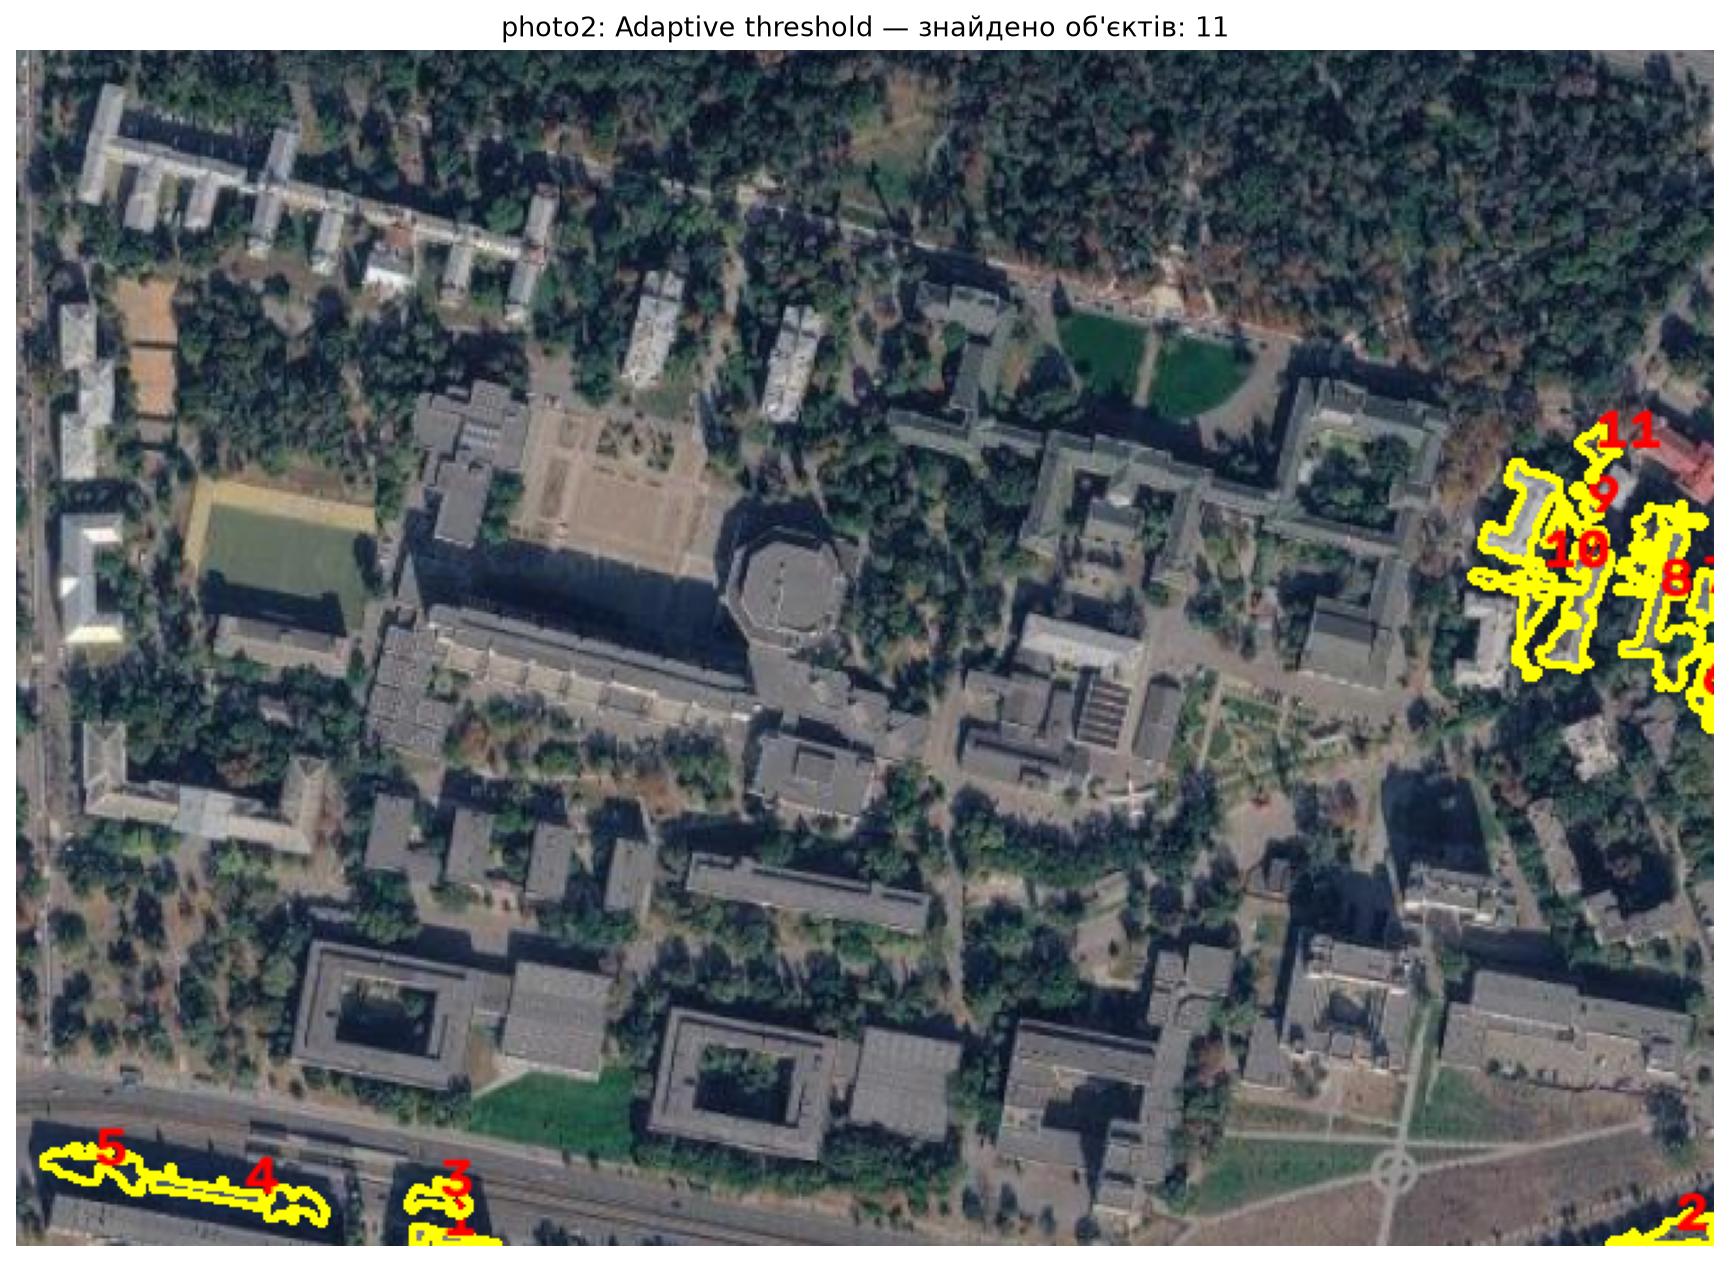
\includegraphics[width=\linewidth]{../results/photo2/adaptive_result.png}\\
    \scriptsize Adaptive: contours
  \end{minipage}

  \vspace{0.45em}
  \begin{minipage}{0.31\textwidth}
    \centering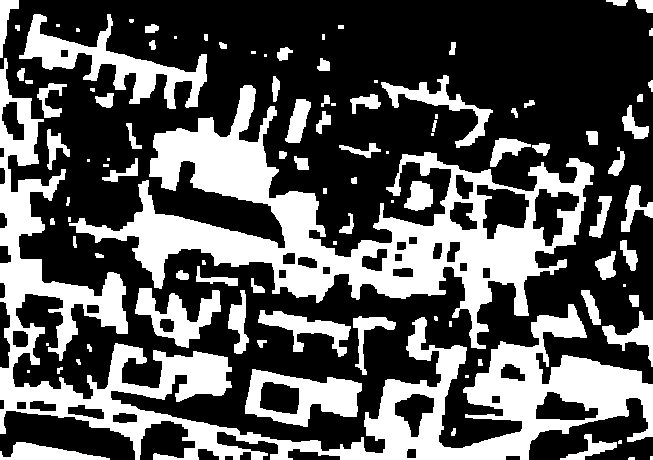
\includegraphics[width=\linewidth]{../results/photo2/color_mask.png}\\
    \scriptsize Color mask
  \end{minipage}\hfill
  \begin{minipage}{0.31\textwidth}
    \centering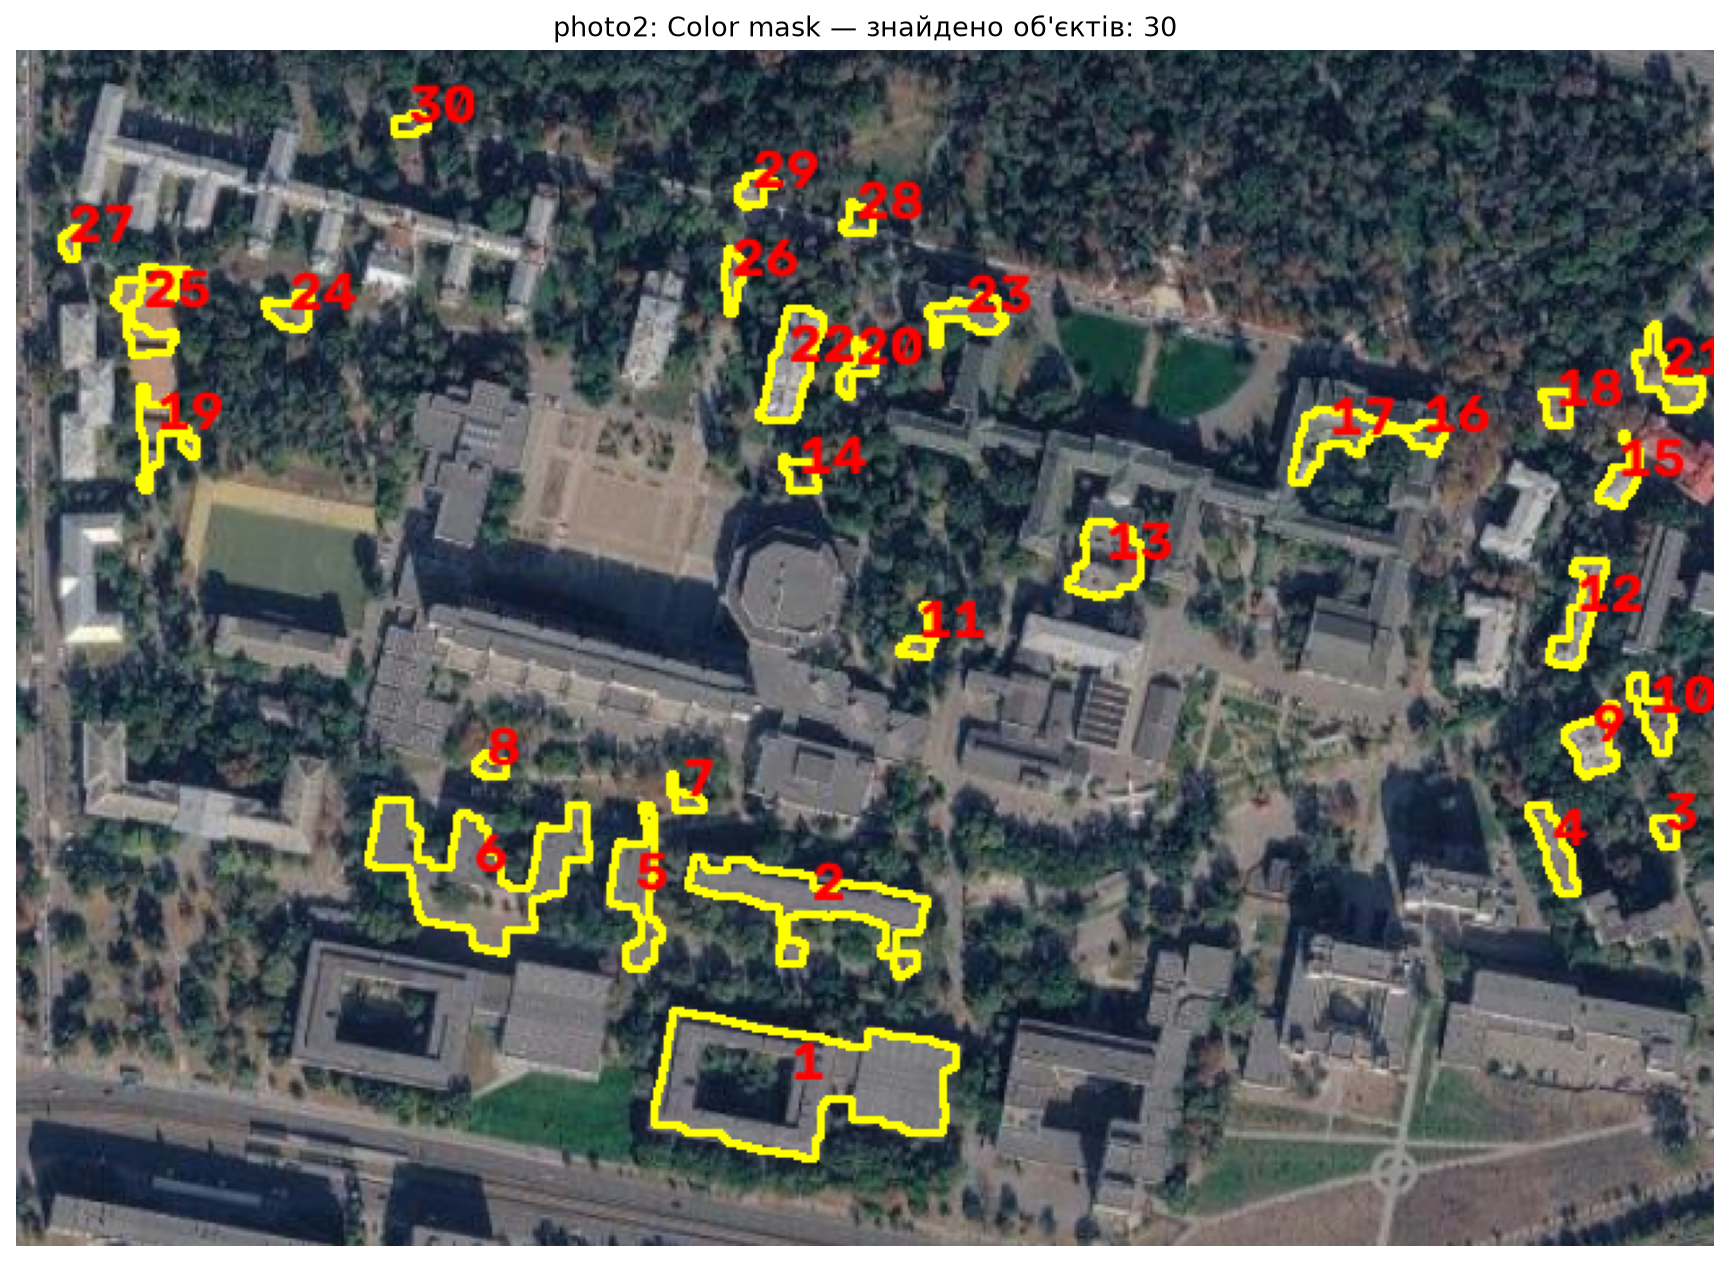
\includegraphics[width=\linewidth]{../results/photo2/color_result.png}\\
    \scriptsize Color: contours
  \end{minipage}\hfill
  \begin{minipage}{0.31\textwidth}
    \centering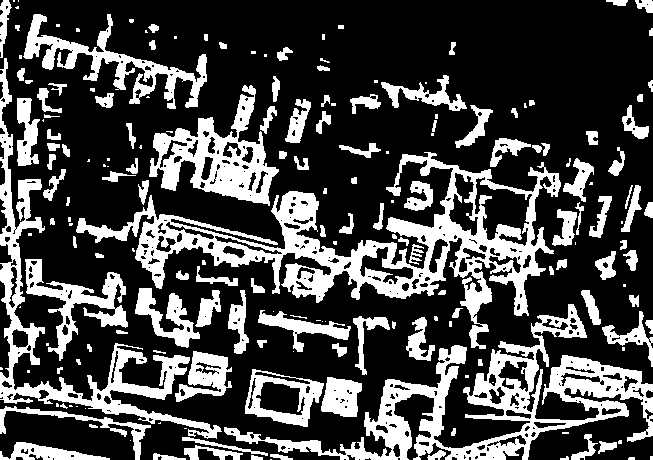
\includegraphics[width=\linewidth]{../results/photo2/consensus_mask.png}\\
    \scriptsize Consensus: mask
  \end{minipage}

  \vspace{0.45em}
  \begin{minipage}{0.31\textwidth}
    \centering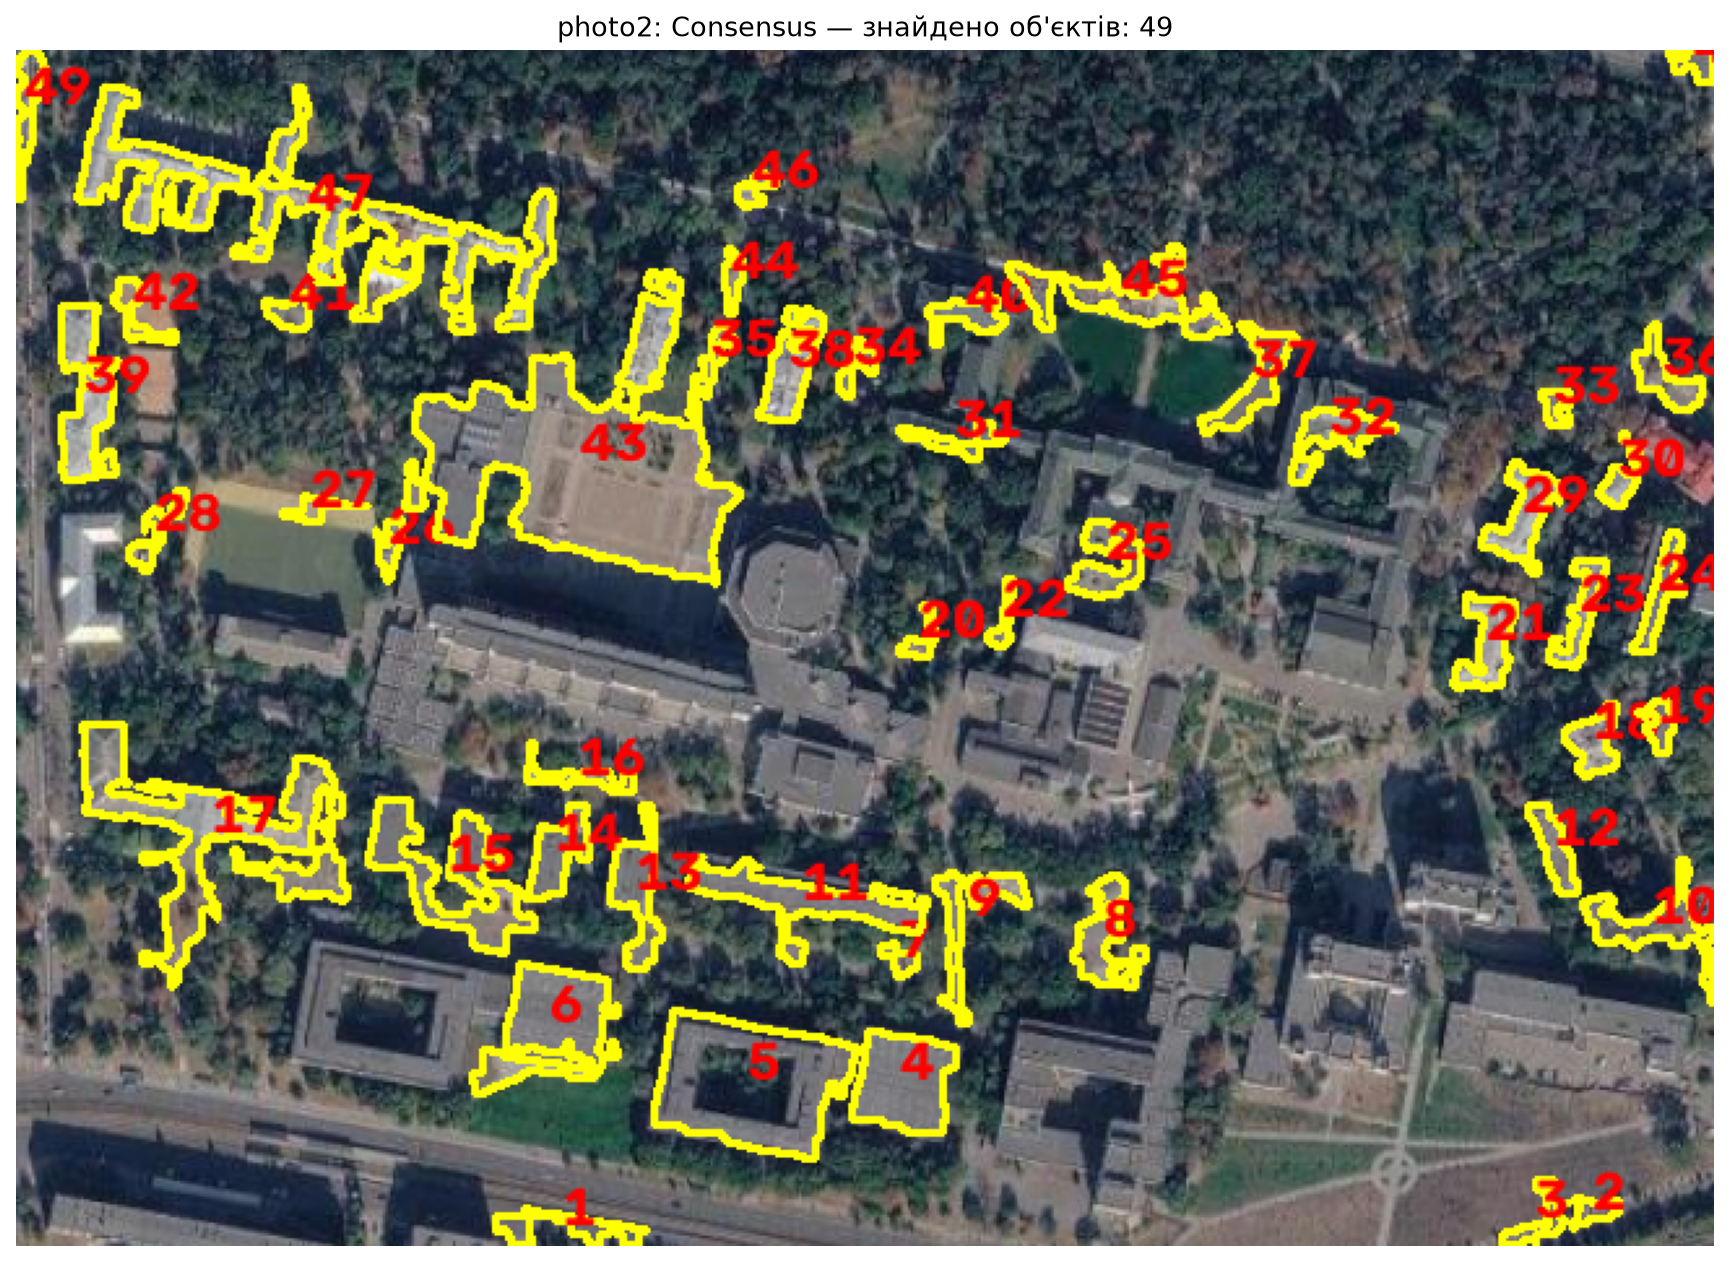
\includegraphics[width=\linewidth]{../results/photo2/consensus_result.png}\\
    \scriptsize Consensus: contours
  \end{minipage}
  \caption{Усі проміжні та фінальні результати для зображення 2}
\end{figure}

Для підвищення надійності два зображення було вирівняно методом ORB. Після ratio test та RANSAC отримано 23 внутрішні відповідності ключових точок. На рисунку показано суміщення зображень.

\begin{figure}[H]
  \centering
  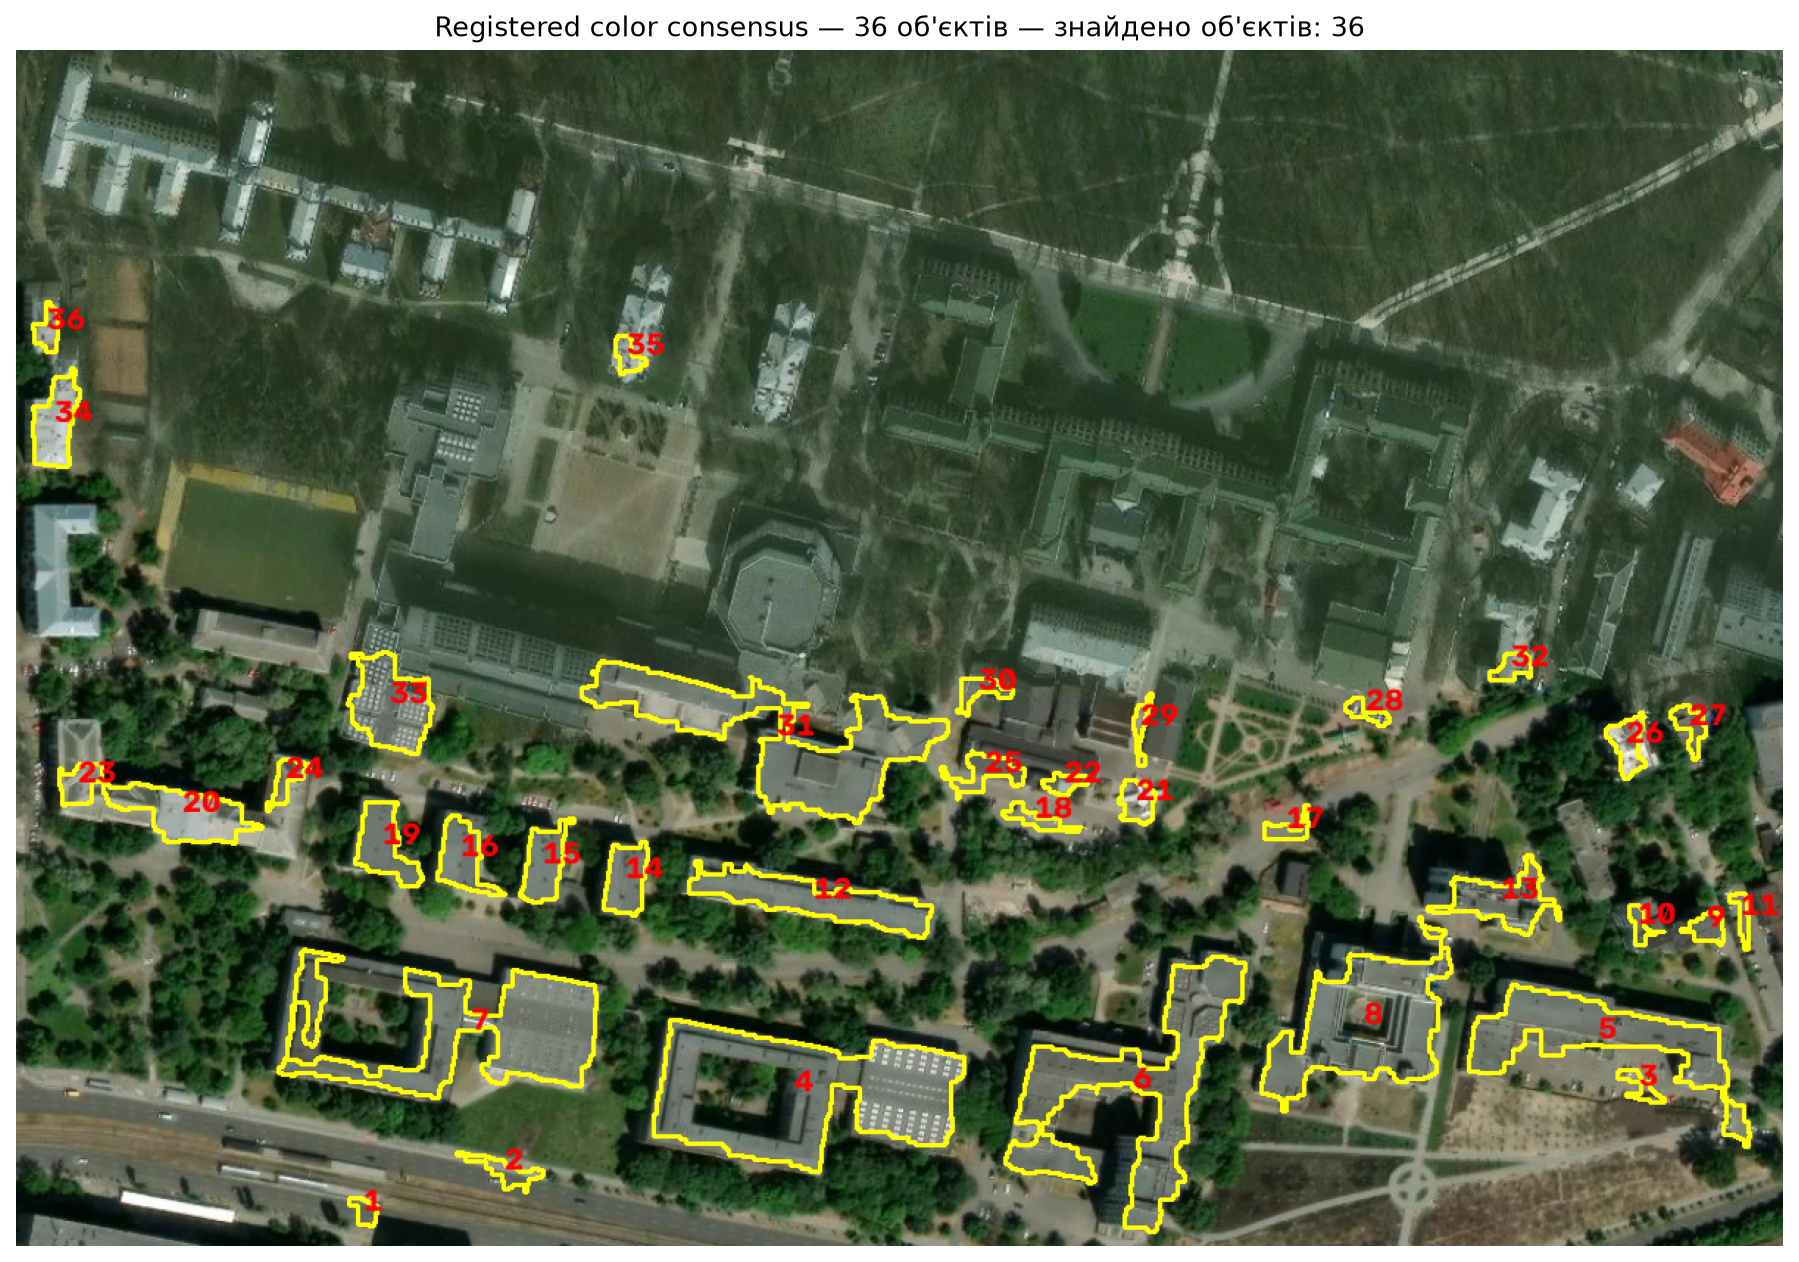
\includegraphics[width=0.92\textwidth]{../results/registered_pair/registered_color_consensus_result.png}
  \caption{Фінальний результат зареєстрованого кольорового консенсусу}
\end{figure}

Після перетину кольорових масок і геометричної фільтрації отримано 36 стабільних кандидатів. Це число не слід трактувати як гарантовано точну кількість будівель: растрові контури можуть відповідати дорогам, дахам, фрагментам споруд або об'єднаним будівлям. Проте перетин двох знімків зменшує кількість випадкових спрацьовувань.

\begin{figure}[H]
  \centering
  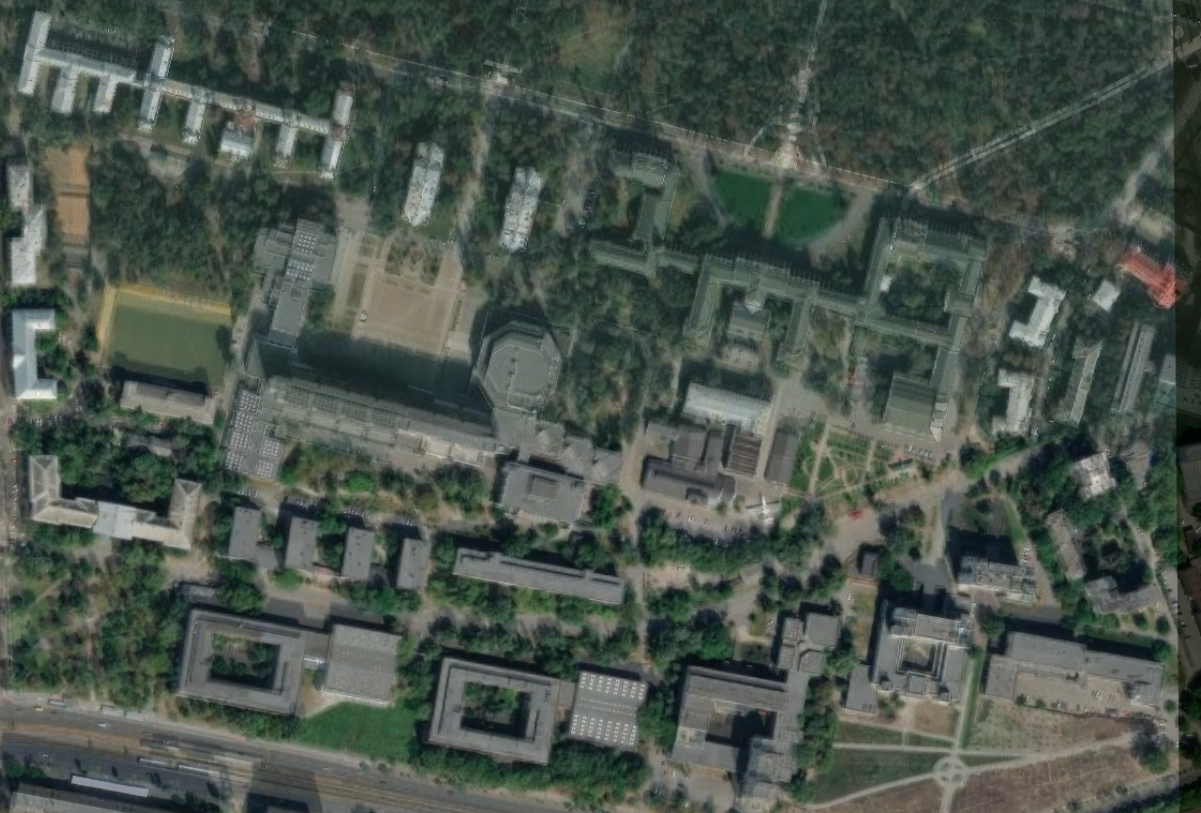
\includegraphics[width=0.92\textwidth]{../results/registered_pair/alignment_blend.png}
  \caption{Результат просторового вирівнювання двох зображень}
\end{figure}

\begin{figure}[H]
  \centering
  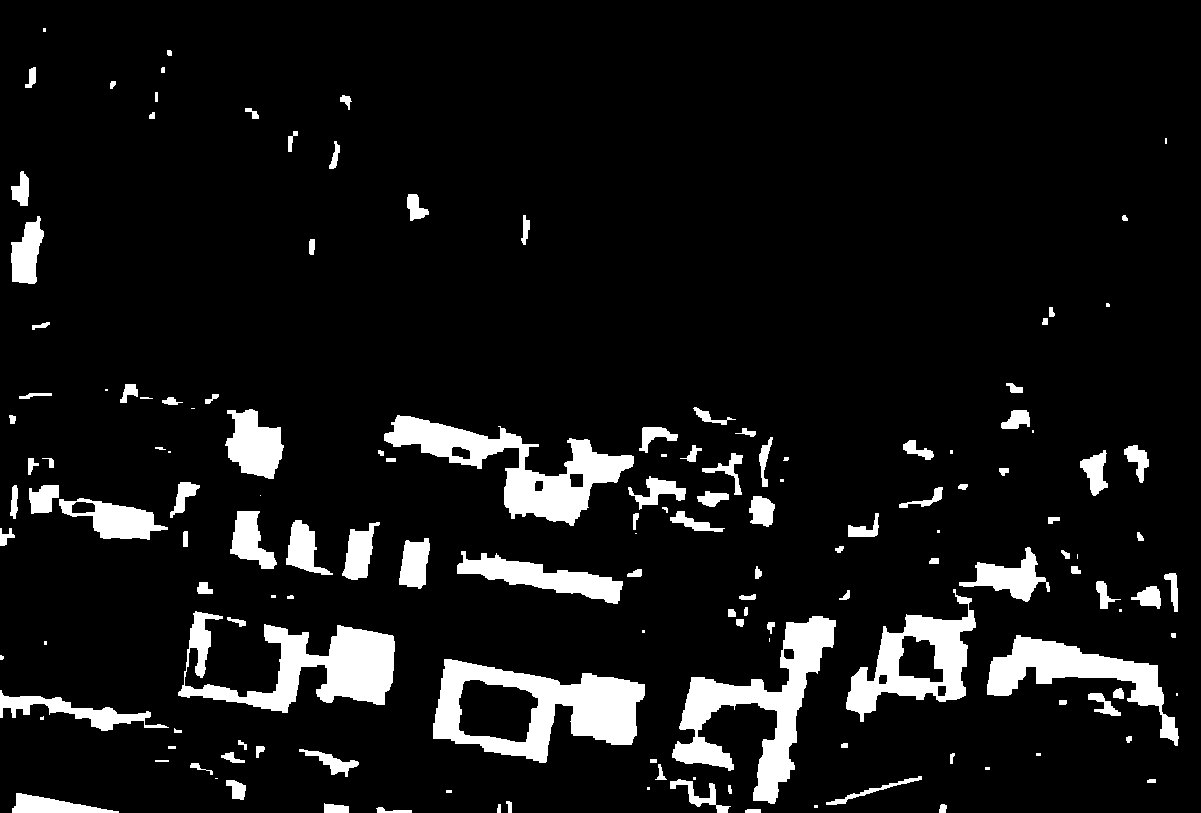
\includegraphics[width=0.92\textwidth]{../results/registered_pair/registered_color_consensus_mask.png}
  \caption{Зареєстрована спільна маска}
\end{figure}

Використані фінальні параметри наведено в таблиці.

\begin{table}[H]
  \centering
  \renewcommand{\arraystretch}{1.2}
  \begin{tabular}{ll}
    \toprule
    \textbf{Параметр} & \textbf{Значення} \\
    \midrule
    Розмір Gaussian blur & \(5\times5\) \\
    Color mask для зображення 1 & \(c=15,\;v=90\) \\
    Color mask для зображення 2 & \(c=20,\;v=110\) \\
    Розмір ядра closing & \(3\times3\) \\
    Мінімальна нормована площа & \(0.0002\) \\
    Максимальна нормована площа & \(0.03\) \\
    Допустиме співвідношення сторін & \(0.20\ldots5.0\) \\
    Мінімальний extent & (0.25) \\
    \bottomrule
  \end{tabular}
  \caption{Фінальна конфігурація фільтрації}
\end{table}

\section{Тестування та верифікація}

Виконано синтаксичну перевірку програмного скрипта та контрольний запуск на двох вхідних зображеннях. Перевірено:

\begin{itemize}[leftmargin=*,itemsep=0.25em]
  \item коректне завантаження обох зображень;
  \item формування всіх проміжних масок;
  \item відсутність помилок під час пошуку контурів;
  \item збереження результатів для кожного pipeline;
  \item знаходження ключових точок ORB і гомографії;
  \item отримання 23 внутрішніх відповідностей під час вирівнювання;
  \item отримання 36 стабільних контурів фінальним pipeline.
\end{itemize}

Для оцінювання повноти виявлення будівель у практичній задачі потрібна еталонна розмітка. Якщо \(TP\) --- кількість правильно знайдених будівель, а \(FN\) --- кількість пропущених, повнота обчислюється як:

\begin{equation}
  Recall=\frac{TP}{TP+FN}\cdot100\%.
\end{equation}

У цій роботі еталонна піксельна розмітка не використовувалася, тому наведені числа є кількістю прийнятих контурів-кандидатів, а не доведеним відсотком правильності.

\section{Фрагменти програмного коду}

Нижче наведено повний код, що забезпечує отримання результатів, та файл залежностей проєкту.

\noindent\textbf{Лістинг 1 --- основний програмний код}

\inputminted{python}{../src/main.py}

\noindent\textbf{Лістинг 2 --- залежності проєкту}

\inputminted{text}{../requirements.txt}

\section{Висновки}

У лабораторній роботі досліджено способи підготовки растрових зображень і векторизації об'єктів за допомогою OpenCV. Реалізовано grayscale, гаусове згладжування, глобальну та адаптивну бінаризацію, Canny, кольорову маску, морфологічне замикання, пошук контурів і геометричну фільтрацію.

Проведене порівняння показало, що Canny не є оптимальним основним методом для цієї задачі, оскільки повертає переважно межі об'єктів і чутливий до якості знімка. Кольорова маска краще підходить для виділення світлих дахів, але також потребує фільтрації хибних спрацьовувань.

Найкращою для досліджуваних знімків виявилася комбінація кольорових масок двох зображень із попереднім ORB-вирівнюванням. Перетин масок залишає стабільні області, що спостерігаються на обох знімках. Фінальний pipeline сформував 36 стабільних контурів-кандидатів. Точність підрахунку може бути додатково підвищена за наявності еталонної розмітки або спеціалізованої моделі сегментації будівель.

\end{document}
